\documentclass[11pt,a4paper]{article}
\usepackage[margin=1in]{geometry}
\usepackage{amsmath,amssymb,amsthm,mathtools}
\usepackage{booktabs,multirow,array}
\usepackage{graphicx}
\usepackage{flafter}
\usepackage{capt-of}
\setlength{\emergencystretch}{2em}
\usepackage{microtype}
\usepackage{enumitem}
\usepackage[colorlinks=true,linkcolor=blue,citecolor=blue,urlcolor=blue]{hyperref}
\usepackage[authoryear,round,sort&compress]{natbib}
% In author-year mode natbib makes \cite behave like \citet; bind it to the
% parenthetical form so that only explicit \citet produces "Author (Year)".
\let\cite\citep

\newtheorem{theorem}{Theorem}
\newtheorem{proposition}[theorem]{Proposition}
\newtheorem{lemma}[theorem]{Lemma}
\newtheorem{corollary}[theorem]{Corollary}
\theoremstyle{definition}
\newtheorem{definition}[theorem]{Definition}
\theoremstyle{remark}
\newtheorem{remark}[theorem]{Remark}

\DeclareMathOperator{\rank}{rank}
\DeclareMathOperator{\cond}{cond}
\DeclareMathOperator{\Var}{Var}
\newcommand{\R}{\mathbb{R}}
\newcommand{\T}{\mathsf{T}}

\title{What ParallaxBA Actually Buys:\\
Better Scaling, Not More Information}
\author{%
  Zhengkang Zuo\thanks{Corresponding author: \texttt{zuozhengkang@tyut.edu.cn}.
  ORCID iD: \href{https://orcid.org/0000-0003-1255-6332}{0000-0003-1255-6332}.}\\[3pt]
  \normalsize Polar-vision Laboratory, College of Geoscience and Surveying Engineering,\\
  \normalsize Taiyuan University of Technology, Taiyuan 030024, Shanxi, China
}
\date{\today}

\begin{document}
\maketitle

\begin{abstract}
Parallax-angle bundle adjustment (ParallaxBA) rests on a chain of inferences: from a positive-definite two-dimensional information matrix to three-dimensional identifiability, and from chart conditioning to problem conditioning and convergence. Checked one at a time, the links do not all hold. The two-dimensional matrix is positive definite, and so is its three-dimensional counterpart on the regular domain, but neither makes depth identifiable: the depth-to-parallax map is non-injective under aligned motion, and at exact collinearity the scaled-ray observation returns the zero vector. The step from chart conditioning to convergence does not follow, because for any chart that smoothly reparameterizes the point coordinates the Schur complement a solver factorizes is identical elementwise --- it is $A^{\T}(I-P)A$, with $P$ projecting onto the column space the points already span --- so only the damping metric and the domain remain free to affect the solve, and neither carries information. What the chart does buy is real: a bounded chart Hessian where XYZ grows as $\omega^{-2}$, and a trust region stretched along depth by $d/B$ at $\beta=\pi/2$. Four charts spanning seven orders of magnitude in $\kappa(H)$ return the same physical Gauss--Newton iterates to $4\times10^{-14}$ and the same depth Cram\'er--Rao bound to $3\times10^{-10}$; on a real handheld sequence the reduced system agrees to $9\times10^{-14}$, and a re-run of the experiment that indicts inverse depth, given the Euclidean control it omits, fails for all three depth-coordinate charts at one threshold. This is a refutation of an argument, not of a method.
\end{abstract}

\vspace{0.6em}
\noindent\textbf{Keywords:} bundle adjustment, parallax parametrization, point coordinates, Schur complement, conditioning, identifiability

\section{Introduction}
Bundle adjustment (BA) estimates camera poses and scene structure by minimizing reprojection error \cite{triggs1999bundle,hartley2004multiple}, and it remains the back end of most modern localization and mapping systems \cite{cadena2016slam}. Although the physical objective is shared, the coordinates used for object points can change a numerical solver's trajectory so drastically that the choice is often treated as a modelling decision rather than an implementation detail: inverse depth accompanies the large depth uncertainty of monocular initialization \cite{civera2008inverse} and of sparse direct formulations \cite{engel2018dso}, XYZ the incremental reconstructions of structure-from-motion \cite{snavely2006photo,schonberger2016sfm}. \citet{zhao2015parallaxba} proposed ParallaxBA, representing a point by a main-anchor bearing and the parallax angle at an associate anchor. Their analysis attributes slow or failed convergence of XYZ and inverse-depth BA to singular or ill-conditioned normal equations and flat objective regions, and reports substantial empirical improvements.

This paper shows that the choice of point coordinates cannot change the problem a solver converges to, only the path it takes, and that this distinction decides a specific published disagreement. The claim under test is therefore narrow, and it is worth stating what it is not. It is not that ParallaxBA performs badly: we confirm, and give a proof of, two mechanisms by which it genuinely helps. It is that the argument offered for it does not support the conclusion drawn, because the quantity it computes is a property of the coordinates and the quantity it concludes about is a property of the problem. Three different claims are routinely conflated at this point:
\begin{enumerate}[leftmargin=2em]
  \item \textbf{Auxiliary-coordinate regularity:} a Jacobian or Gauss--Newton matrix is full rank in a chosen coordinate system;
  \item \textbf{Physical identifiability:} the image observations determine a finite Euclidean point, including its depth;
  \item \textbf{Algorithmic performance:} a particular GN/LM implementation reaches an acceptable objective value within a finite budget.
\end{enumerate}
The first does not imply the second unless the coordinate transformation is locally regular. Neither automatically implies the third, which also depends on damping, scaling, initialization, stopping rules, linear algebra, and the iteration budget.

The empirical literature is likewise mixed. The original ParallaxBA paper reports better convergence in most of its experiments while explicitly disclaiming universal convergence guarantees \cite{zhao2015parallaxba}. \citet{zuo2023applicability} subsequently questioned its suitability for three-dimensional short-baseline photography. Manifold-based PMBA extends the representation and introduces a different objective and initialization scheme \cite{liu2018pmba}; it is not covered by counterexamples directed at the original ParallaxBA equation. A useful analysis must therefore avoid both overstatements: ``parallax eliminates the relevant singularities everywhere'' and ``parallax is generally ineffective in three-dimensional BA.''

\subsection{What is inherited, and what is new}
The invariance of the normal equations under reparameterization is classical. \citet{triggs1999bundle} present the Schur complement as the object a bundle adjuster actually factorizes and observe that the choice of point coordinates changes the conditioning of that reduced system without changing its stationary points; \citet{bartoli2003gauge} shows that gauge-dependent damping, rather than the linearization, is what makes Levenberg--Marquardt behave differently in different gauges, and construct a gauge-invariant alternative.

We inherit both observations and claim neither. What is new is narrower, and we argue that it is decisive. First, the charts compared here depend on the \emph{optimized anchor poses}, so the change of variables is state-dependent and the classical fixed-reparameterization argument does not apply directly; Theorem~\ref{thm:main} shows that the Schur complement is nevertheless identical elementwise. Second, we give the rank bookkeeping $\rank\mathcal S=\rank H-\rank J_X$, which makes the consequence explicit: a singular point block is neither necessary nor sufficient for a singular reduced camera system, so point-block conditioning cannot support any conclusion about BA singularity in either direction. Third, we apply this to a published argument and to the experiments offered in its support, including a re-run of the experiment that indicts inverse depth with the control it omits.

\subsection{Contributions}
This paper offers a mathematical and empirical reconciliation. The mathematics has one job --- to name the object that a solver factorizes and show that the chart does not appear in it --- and the experiments have one job --- to check that claim where depth error is measurable. Everything else follows from these two.
\begin{itemize}[leftmargin=2em]
  \item A chart theorem at the bundle-adjustment level. The reduced camera matrix is identical elementwise across regular charts, anchor coupling cancels exactly, and $\rank\mathcal S=\rank H-\rank J_X$. A singular point block is therefore neither necessary nor sufficient for BA singularity, so point-block conditioning cannot support a conclusion about singularity in either direction. The only surviving differences are the damping metric and the domain.
  \item An application that separates what the original proof establishes from what was inferred. Its $2\times2$ information matrix is positive definite and correct; the three-dimensional corollary is not, because the depth-to-parallax map is non-injective under aligned motion and the scaled-ray observation returns the zero vector at exact collinearity.
  \item A positive answer to what the chart is worth, since refuting an argument is only half the question. The chart Hessian stays bounded while the XYZ one grows as $\omega^{-2}$, which is a preconditioning of the depth direction; at $\beta=\pi/2$ the trust region is stretched along depth by $d/B$, which is a geometry of damping. Neither adds an observation, and both are worth having.
  \item A normalized complementary chart that removes the zero ray at alignment, together with a proof that it changes the admissible set and not the information.
  \item Controlled synthetic problems with known depth, in which four charts spanning seven orders of magnitude in $\kappa(H)$ return the same iterates, the same depth Cram\'er--Rao bound, and the same physical rank loss; and a re-run of the experiment that indicts inverse depth, supplied with the Euclidean control it omits.
  \item Two tests on a real handheld sequence, one for the equality and one for the depth error, so that neither conclusion rests on a rig we designed.
\end{itemize}

\section{Related Work}
Inverse-depth parametrization was developed for undelayed monocular EKF initialization and for representing large depth uncertainty, including points at infinity \cite{civera2008inverse}. It remains the standard choice wherever that uncertainty is the organizing problem, from filter-based monocular SLAM \cite{strasdat2010scaledrift,murartal2015orbslam} to sparse direct formulations \cite{engel2018dso}. Optical-axis inverse depth $1/z$ and inverse Euclidean range $1/\|x\|$ are distinct coordinates, and the four charts compared below include both, so the ambiguity between them can be kept out of the experiments.

ParallaxBA instead uses two anchor cameras and a parallax angle \cite{zhao2015parallaxba}, a representation its authors reached from a linear formulation of the same estimation problem \cite{zhao2014linear}. An earlier study led by the present author \cite{zuo2023applicability} extended parts of the sensitivity discussion to three dimensions and reported unfavorable short-baseline simulations and two small real SfM experiments. That study is the immediate precursor of this paper, and what follows revises part of its reasoning rather than its measurements; we therefore make no claim to be the first to question a two-dimensional-to-three-dimensional extrapolation. Our distinct focus is the exact scaled-ray domain, chart regularity, matched initial physical states, and a much larger controlled BA comparison.

PMBA uses manifold ray coordinates and a modified observation-ray objective \cite{liu2018pmba}. Those changes can alter the relevant singular sets. The counterexample in Section~\ref{sec:zero-ray} is therefore specific to the original ParallaxBA scaled-ray equation and implementations that reproduce it.

Whatever the chart, the same machinery consumes it. Production bundle adjusters eliminate the points and factorize a reduced camera system \cite{lourakis2009sba}, whether through a general graph-optimization front end \cite{kummerle2011g2o} or a differentiable least-squares library \cite{ceres2023}. That shared architecture is what makes the question of this paper well posed, and it is also why an answer that holds only for one implementation would be of little use.

Gauge-dependent LM damping has long been studied in BA. The algorithm itself dates to \citet{marquardt1963}, with the trust-region reading and implementation guidance of \citet{more1978}; \citet{lourakis2005lm} compare it against alternatives for bundle adjustment specifically. \citet{bartoli2003gauge} showed that a sufficiently general damping matrix can reproduce a gauge transformation and enable gauge-invariant iterations. Our pullback-metric statement is an application of the same general optimization principle, rather than a new claim that arbitrary damped iterations are coordinate invariant. Standard treatments of GN/LM similarly emphasize the role of the trust-region metric \cite{nocedal2006numerical}.

\section{A Reparameterization Framework}
\label{sec:framework}
Let $r(x)\in\R^m$ be a physical residual vector and let $x=g(q)$ be a local coordinate transformation. On a common open set, assume that
\begin{equation}
  D(q) := \frac{\partial g}{\partial q}
\end{equation}
exists, is square, and is nonsingular. Define
\begin{equation}
  J_x=\frac{\partial r}{\partial x},\qquad
  J_q=\frac{\partial r(g(q))}{\partial q}=J_xD.
\end{equation}
For a common residual weighting, let $H_x=J_x^\T WJ_x$, $g_x=J_x^\T Wr$, and analogously in $q$.

\begin{theorem}[Physical GN step invariance]
\label{thm:gn}
If $D$ and $H_x$ are nonsingular at the current point, the GN steps satisfy
\begin{equation}
  \boxed{\delta x=D\,\delta q.}
\end{equation}
Thus, the two coordinate systems generate the same physical GN linearization step.
\end{theorem}
\begin{proof}
The $q$-coordinate normal equations are
\begin{align}
  (D^\T H_xD)\delta q
    &=-D^\T g_x.
\end{align}
Premultiplying the $x$-coordinate solution $\delta x=-H_x^{-1}g_x$ by $D^\T H_x$ gives
$D^\T H_x\delta x=-D^\T g_x$. Substitution of $\delta x=D\delta q$ yields the $q$ equation; nonsingularity makes the solution unique.
\end{proof}

\begin{corollary}[No new stationary points on a regular chart]
Stationary points and attainable local minimizers correspond under $g$ on the common open chart. A change of coordinates alone cannot create additional physical image information or change the underlying reprojection objective.
\end{corollary}

\begin{proposition}[LM invariance requires a pullback metric]
\label{prop:lm}
Let the $q$-coordinate LM step use $\lambda I$. If the $x$-coordinate step uses
\begin{equation}
  M_x=(DD^\T)^{-1},
\end{equation}
then $(H_q+\lambda I)\delta q=-g_q$ and $(H_x+\lambda M_x)\delta x=-g_x$ are equivalent under $\delta x=D\delta q$.
\end{proposition}
\begin{proof}
Substitute $\delta x=D\delta q$ and premultiply the $x$ equation by $D^\T$. The damping term becomes
\begin{equation}
  \lambda D^\T(DD^\T)^{-1}D\,\delta q=\lambda\delta q,
\end{equation}
which gives precisely the $q$-coordinate LM equation.
\end{proof}

Using $\lambda I$ in both charts generally compares different physical trust regions. Different convergence trajectories are therefore entirely compatible with Theorem~\ref{thm:gn}. Conversely, raw conditioning is not invariant:
\begin{equation}
  H_q=D^\T H_xD,
\end{equation}
so $\cond(H_q)$ and $\cond(H_x)$ can differ without changing the physical GN step. In the scalar depth/inverse-depth example used below, diagonal column normalization makes the two $2\times2$ correlation matrices identical, even though their unscaled condition numbers differ by orders of magnitude. This local observation does not assert that full BA Jacobians become identical after column normalization.

For Gaussian measurement noise, Fisher information transforms by the same pullback:
\begin{equation}
  \mathcal I_q=D^\T\mathcal I_xD.
  \label{eq:fisher}
\end{equation}
If $D$ is singular, a full-rank auxiliary matrix cannot be pulled back to a nonsingular physical information matrix. This is the key distinction needed for the aligned ParallaxBA example. Theorem~\ref{thm:gn} is the block-level statement for a constant $D$. Section~\ref{sec:ba-theorem} extends it to the whole BA problem, where $D$ becomes a block triangular $T$ that depends on the optimized poses and the points are eliminated by a Schur complement.

\section{A Chart Theorem at the Bundle-Adjustment Level}
\label{sec:ba-theorem}

The three claims distinguished in the introduction can be separated only once the object that a solver actually factorizes has been named. A reader sympathetic to ParallaxBA can reasonably object that a single feature is not a bundle adjustment: BA couples $n$ poses and $m$ points, the solver eliminates the points through a Schur complement, and the anchor poses are themselves optimized variables. Three objections follow.
\begin{enumerate}[leftmargin=2em]
  \item A singular point block need not make the reduced camera system singular, because the Schur complement discards exactly those directions that the points can absorb.
  \item The chart depends on the anchor poses, so a change of point coordinates is not a fixed reparameterization and the usual invariance argument may fail.
  \item Even if the undamped linearization is invariant, Levenberg--Marquardt traverses different trust regions in different coordinates, so a damped trajectory may differ.
\end{enumerate}
This section settles all three; Theorem~\ref{thm:main} is the outcome. The first objection is correct, and it is the precise reason why point-block conditioning is the wrong diagnostic for BA. The second does not rescue the original claim. The third identifies the only place where a genuine and provable numerical advantage survives.

\subsection{Chart family and the total-space map}
\label{sec:chart-family}

Let the problem have $n$ cameras with world-to-camera rotations $R_i$ and optical centres $c_i$, and $m$ points $X_j$. Write $\xi=(\xi_1,\dots,\xi_n)$ with $\xi_i=(R_i,c_i)$ and $X=(X_1,\dots,X_m)$. The residual of observation $(i,j)$ and the objective are
\begin{equation}
r_{ij}(\xi_i,X_j)=\pi\!\left(R_i(X_j-c_i)\right)-u_{ij}\in\R^2,
\qquad
F(\xi,X)=\tfrac12\|r(\xi,X)\|^2,
\label{eq:ba-residual}
\end{equation}
with $\pi(x,y,z)=(x/z,\,y/z)$.

For each point $j$, let $m(j)$ and $a(j)$ be two cameras that observe it, write $C_m=c_{m(j)}$, $C_a=c_{a(j)}$, and set $b_j=C_a-C_m$, $B_j=\|b_j\|>0$, $\hat b_j=b_j/B_j$. Let $n_j$ be the unit main-anchor bearing, $\beta_j=\angle(n_j,\hat b_j)$, and let $\alpha_j$ be the azimuth of $n_j$ about $\hat b_j$. With $\omega_j=\angle(C_mX_jC_a)$ the parallax angle at the point, the sine law in the triangle $C_mC_aX_j$ gives
\begin{equation}
d_j=\frac{B_j\sin(\beta_j+\omega_j)}{\sin\omega_j},
\qquad
X_j=\Phi_\xi(q_j):=C_m+d_j\,n_j(\beta_j,\alpha_j),
\qquad
q_j=(\alpha_j,\beta_j,\omega_j).
\label{eq:chart}
\end{equation}
This is the same sine law as Equation~\eqref{eq:sine-law}, written with $\beta_j$ for the angle there denoted $\phi_j$ and with $B_j=\|t_a-t_m\|$; the difference is that \eqref{eq:chart} is now read as a chart on the point coordinates rather than as a formula for a scalar depth.

Two features of \eqref{eq:chart} matter below. First, $\Phi_\xi$ depends on $\xi$, because the anchor centres are optimization variables; the map is a chart on the fibre over $\xi$, not a global change of variables. Second, its Jacobian degenerates on a set larger than the zero-parallax ray. Differentiating at fixed $\xi$,
\begin{equation}
\partial_{\alpha}\Phi=d\sin\beta\,\hat\alpha,\qquad
\partial_{\beta}\Phi=\frac{B\cos(\beta+\omega)}{\sin\omega}\,n+d\,u,\qquad
\partial_{\omega}\Phi=-\frac{B\sin\beta}{\sin^{2}\omega}\,n,
\label{eq:chart-columns}
\end{equation}
where $u=\partial_\beta n$ and $\hat\alpha=\partial_\alpha n/\sin\beta$, so that
\begin{equation}
\det D_q=-\frac{B\,d^{2}\sin^{2}\beta}{\sin^{2}\omega},
\qquad D_q=\frac{\partial\Phi}{\partial q}.
\label{eq:chart-det}
\end{equation}
The chart is therefore a local diffeomorphism wherever $\det D_q\neq0$, and it represents a positive-depth point with a defined main ray exactly on
\begin{equation}
\mathcal D=\{\sin\beta\neq0,\ \sin\omega\neq0,\ \beta+\omega<\pi\},
\label{eq:chart-domain}
\end{equation}
the last inequality being precisely $d>0$.

Collecting poses and chart coordinates, define the total-space map and its Jacobian
\begin{equation}
\Psi(\xi,q)=(\xi,\Phi_\xi(q)),
\qquad
T=\frac{\partial(\xi,X)}{\partial(\xi,q)}
=\begin{bmatrix}I&0\\G&D_q\end{bmatrix},
\qquad
G=\frac{\partial\Phi_\xi(q)}{\partial\xi}.
\label{eq:T}
\end{equation}
Because $T$ is block upper triangular with diagonal blocks $I$ and $D_q$,
\begin{equation}
\det T=\prod_{j}\det D_{q,j},
\qquad
T^{-1}=\begin{bmatrix}I&0\\-D_q^{-1}G&D_q^{-1}\end{bmatrix}.
\label{eq:T-inverse}
\end{equation}
Throughout this section we assume the following.

\smallskip
\noindent\textbf{(R) Regular linearization.} At the linearization point every $3\times3$ block $D_{q,j}$ is invertible, that is, the linearization point lies in $\mathcal D^{m}$.

\subsection{The chart is a congruence in the total space}
\label{sec:congruence}

\begin{theorem}[Total-space congruence]\label{thm:congruence}
Let (R) hold, let $J_x=[\,A\ \ J_X\,]$ with $A=\partial r/\partial\xi$ and $J_X=\partial r/\partial X$, let $J_q=\partial r(\xi,\Phi_\xi(q))/\partial q$, and let $H_x=J_x^{\T}J_x$, $g_x=J_x^{\T}r$, with $H_q$ and $g_q$ defined analogously. Then
\begin{equation}
J_q=J_xT,\qquad H_q=T^{\T}H_xT,\qquad g_q=T^{\T}g_x .
\label{eq:congruence}
\end{equation}
Consequently
\begin{enumerate}[label=(\roman*),leftmargin=2.4em]
  \item $\rank H_q=\rank H_x$, and $H_q$ and $H_x$ have the same inertia;
  \item $\ker H_q=T^{-1}\ker H_x$;
  \item $g_q=0\iff g_x=0$, so stationary points correspond one-to-one under $\Psi$;
  \item at a stationary point the exact Hessians satisfy $\nabla^2_q\tilde F=T^{\T}(\nabla^2_xF)T$, where $\tilde F=F\circ\Psi$;
  \item after gauge fixing, $\delta q=T^{-1}\delta x$.
\end{enumerate}
\end{theorem}
\begin{proof}
The chain rule gives $J_q=J_xT$, hence $H_q=T^{\T}J_x^{\T}J_xT=T^{\T}H_xT$ and $g_q=T^{\T}J_x^{\T}r=T^{\T}g_x$. By \eqref{eq:T-inverse} and (R), $\det T=\prod_j\det D_{q,j}\neq0$, so $T$ is invertible.

(i) Congruence preserves rank, and Sylvester's law of inertia preserves the signature of a symmetric matrix. (ii) $H_xv=0$ implies $H_q(T^{-1}v)=T^{\T}H_xv=0$, and conversely. (iii) $T$ is invertible. (iv) Differentiating $\tilde F=F\circ\Psi$ twice gives $\nabla^2\tilde F=T^{\T}(\nabla^2F)T+\sum_k(\nabla F)_k\nabla^2\Psi_k$, and the second term vanishes where $\nabla F=0$. (v) Substitute \eqref{eq:congruence} into $-H_q^{-1}g_q$ and use invertibility of $T$.
\end{proof}

\begin{remark}[Anchor dependence is not an obstruction]\label{rem:anchors}
A natural objection is that Parallax coordinates are not a reparameterization at all, because the chart moves when the anchors move. Theorem~\ref{thm:congruence} shows otherwise. The only requirement is that $T$ be invertible, and $T$ is block upper triangular with $\det T=\prod_j\det D_{q,j}$, independently of $G$. The coupling may be arbitrarily large without affecting \eqref{eq:congruence}: $\Psi$ reparameterizes each fibre $X=\Phi_\xi(q)$ over a fixed $\xi$ while leaving $\xi$ untouched, and a congruence does not require a block-diagonal transformation.
\end{remark}

Exactly two things can break the conclusion: $D_q$ singular, so that $T$ is not invertible and $\Psi$ is not a local diffeomorphism; or a residual that is not the same function of the physical point. The second does not apply to implementations that project the scaled ray, since $\sin\omega\,(X-C_a)$ and $X-C_a$ differ by a positive scale and therefore have the same perspective projection whenever $\sin\omega>0$. The first applies on the complement of $\mathcal D$, and Section~\ref{sec:zero-ray} shows that this complement is nonempty and physically realizable.

\subsection{Point-block singularity and the reduced camera system}
\label{sec:schur}

Bundle adjustment does not solve \eqref{eq:congruence} directly: it eliminates the points and solves a reduced camera system. A singular point block might therefore be harmless, and making this precise also explains why a positive-definite point block cannot certify the camera system. Partition
\begin{equation}
H=\begin{bmatrix}H_{pp}&H_{pl}\\H_{lp}&H_{ll}\end{bmatrix}
=\begin{bmatrix}A^{\T}A&A^{\T}J_X\\J_X^{\T}A&J_X^{\T}J_X\end{bmatrix},
\qquad
\mathcal S=H_{pp}-H_{pl}H_{ll}^{+}H_{lp}.
\label{eq:partition}
\end{equation}

\begin{lemma}[Schur complement as a projection]\label{lem:schur}
If $H_{ll}=J_X^{\T}J_X$ then
\begin{equation}
\mathcal S=A^{\T}(I-P_{J_X})A,
\qquad
P_{J_X}=J_X(J_X^{\T}J_X)^{+}J_X^{\T}.
\label{eq:schur-projection}
\end{equation}
\end{lemma}
\begin{proof}
$J_X(J_X^{\T}J_X)^{+}J_X^{\T}$ is the orthogonal projector onto $\operatorname{range}(J_X)$; substituting into \eqref{eq:partition} and using $J_X^{\T}(I-P_{J_X})=0$ gives \eqref{eq:schur-projection}.
\end{proof}

Identity \eqref{eq:schur-projection} is the most useful formula in this paper: it writes the Schur complement as the camera information that survives after removing every direction the points can explain.

\begin{theorem}[Point-block isolation]\label{thm:schur}
With $p=6n$ pose coordinates and $l=3m$ point coordinates,
\begin{equation}
\rank\mathcal S=\rank H-\rank J_X,
\label{eq:rank-identity}
\end{equation}
and
\begin{equation}
\ker H=\{(v,-J_X^{+}Av):v\in\ker\mathcal S\}\oplus\{(0,u):u\in\ker J_X\},
\qquad
\ker\mathcal S=\Pi_\xi\ker H,
\label{eq:kernel-split}
\end{equation}
where $\Pi_\xi$ projects onto the pose coordinates.
\end{theorem}
\begin{proof}
Since $A^{\T}(I-P_{J_X})A\succeq0$, we have $v\in\ker\mathcal S\iff(I-P_{J_X})Av=0\iff Av\in\operatorname{range}J_X$. If $(v,w)\in\ker H$ then $Av+J_Xw=0$, so $Av\in\operatorname{range}J_X$ and $v\in\ker\mathcal S$, while the general solution of $J_Xw=-Av$ is $w=-J_X^{+}Av+u$ with $u\in\ker J_X$. Conversely, for $v\in\ker\mathcal S$ the choice $w=-J_X^{+}Av$ gives $Av+J_Xw=0$. This proves the first identity in \eqref{eq:kernel-split}; the second follows because $(v,w)\mapsto v$ has image $\ker\mathcal S$ and kernel $\{(0,u)\}$. Taking dimensions gives $\dim\ker H=\dim\ker\mathcal S+\dim\ker J_X$, and substituting $p+l-\rank H=(p-\rank\mathcal S)+(l-\rank J_X)$ yields \eqref{eq:rank-identity}.
\end{proof}

\begin{corollary}[Three fates of a singular point block]\label{cor:fates}
Let $u\in\ker J_X$ and $v\in\ker\mathcal S$.
\begin{enumerate}[label=(\roman*),leftmargin=2.4em]
  \item A zero direction $(0,u)$ with $u\neq0$ lowers $\rank H$ and $\rank J_X$ by one each and leaves $\rank\mathcal S$ unchanged. The point is free; the cameras are not affected.
  \item If $Av\neq0$ then $v$ is a coupled zero direction: cameras and points can move together without changing any residual, and $\rank\mathcal S$ drops. This is a genuine BA degeneracy, independent of whether the point block is positive definite.
  \item If the chart degenerates so that a column of $D_q$ vanishes, the corresponding unit vector $e_k$ lies in $\ker J_X$ and case (i) applies. The reduced system is unchanged, but $T$ is singular and Theorem~\ref{thm:congruence} no longer identifies the two problems.
\end{enumerate}
\end{corollary}

The decisive consequence for the original claim is stronger than equality of rank.

\begin{corollary}[Exact invariance of the reduced system]\label{cor:reduced}
Under (R),
\begin{equation}
\mathcal S_q=\mathcal S_x\ \text{elementwise},
\qquad
A_q^{\T}(I-P_{J_X})r=A^{\T}(I-P_{J_X})r .
\label{eq:reduced-invariance}
\end{equation}
Hence the reduced camera step, and with it the complete undamped Gauss--Newton step, coincides in the two charts.
\end{corollary}
\begin{proof}
Let $J_{X,q}=J_XD_q$ and $A_q=A+J_XG$. Invertibility of $D_q$ gives $\operatorname{range}(J_{X,q})=\operatorname{range}(J_X)$ and hence $P_{J_{X,q}}=P_{J_X}$, while $(I-P_{J_X})J_X=0$. Therefore $\mathcal S_q=(A+J_XG)^{\T}(I-P_{J_X})(A+J_XG)=A^{\T}(I-P_{J_X})A$, every cross term vanishing. The reduced gradient is treated identically.
\end{proof}

The point step closes the argument. In chart coordinates
\begin{equation}
\delta q_q=-(J_{X,q}^{\T}J_{X,q})^{+}J_{X,q}^{\T}\left(r+A_q\delta\xi\right),
\end{equation}
and mapping back, using $A_q\delta\xi=A\delta\xi+J_XG\delta\xi$ and $(J_X^{\T}J_X)^{+}J_X^{\T}J_X=I$ on $\operatorname{row}(J_X)$,
\begin{equation}
D_q\delta q_q=-(J_X^{\T}J_X)^{+}J_X^{\T}(r+A\delta\xi)-G\delta\xi .
\label{eq:point-backsub}
\end{equation}
The motion of the chart itself therefore cancels exactly:
\begin{equation}
G\delta\xi+D_q\delta q_q=-(J_X^{\T}J_X)^{+}J_X^{\T}(r+A\delta\xi)=\delta q_x,
\label{eq:cancel}
\end{equation}
so $X_{\rm new}=\Phi_{\xi+\delta\xi}(q+\delta q_q)=X+\delta q_x$, and the full undamped step is pointwise identical.

\paragraph{An exactly collinear point.}
Take four cameras at $(0,0,0)$, $(1,0,0)$, $(0,1,0)$, $(0,0,1)$, five generic points, and one point $X_5=(2,0,0)$ on the ray through the first two centres, observed only by them. Supplementary Table~S1 confirms \eqref{eq:rank-identity} and Corollary~\ref{cor:fates}: the new point adds three columns of which two are independent (its block has singular values $1.149$, $1.133$, $2.36\times10^{-18}$), so $\rank J_X$ and $\rank H$ each rise by two, $\dim\ker H$ rises by one, and $\rank\mathcal S$ does not move. The extra null vector is a pure point direction: the pose part of the eight-dimensional null space has rank seven, and the principal angle between the null spaces of $\mathcal S$ before and after is zero.

% moved to the supplementary material as Table S1

The same configuration exposes the cost of the chart. XYZ keeps a well-defined, if rank-deficient, block. The parallax chart cannot represent $X_5$ at all: every $X_t=(t,0,0)$ with $t>1$ gives $\beta=\omega=0$, and \eqref{eq:chart} evaluates to $0/0$. This is a restriction of the domain, not an advantage of the coordinates.

\subsection{Damping, trust region, and the surviving advantage}
\label{sec:damping}

Theorem~\ref{thm:congruence} concerns the undamped step. Levenberg--Marquardt instead solves
\begin{equation}
(H_q+\lambda I)\delta q=-g_q
\label{eq:lm-q}
\end{equation}
in chart coordinates. Mapping \eqref{eq:lm-q} with \eqref{eq:congruence} and $\delta x=T\delta q$ gives
\begin{equation}
\left(H_x+\lambda T^{-\T}T^{-1}\right)\delta x=-g_x .
\label{eq:lm-x}
\end{equation}

\begin{theorem}[Damping metric]\label{thm:damping}
The isotropic damping $\lambda I$ in chart coordinates is the anisotropic damping $\lambda M$ in physical coordinates, with
\begin{equation}
M=T^{-\T}T^{-1}
=\begin{bmatrix}
I+G^{\T}D_q^{-\T}D_q^{-1}G & -G^{\T}D_q^{-\T}D_q^{-1}\\
-D_q^{-\T}D_q^{-1}G & D_q^{-\T}D_q^{-1}
\end{bmatrix}.
\label{eq:metric}
\end{equation}
For fixed anchors, $G=0$ and $M=\operatorname{diag}\!\left(I,(D_qD_q^{\T})^{-1}\right)$.
\end{theorem}
\begin{proof}
Premultiply \eqref{eq:lm-q} by $T^{-\T}$, insert $H_q=T^{\T}H_xT$, $g_q=T^{\T}g_x$ and $\delta q=T^{-1}\delta x$, and compare with \eqref{eq:lm-x}. Equation~\eqref{eq:metric} follows by inverting \eqref{eq:T-inverse}.
\end{proof}

Two charts using $\lambda I$ therefore explore different families of trust-region ellipsoids and can follow different damped trajectories, even though their undamped steps coincide. The difference is accounted for entirely by \eqref{eq:metric} and vanishes as $\lambda\to0$; it is not an information difference.

At fixed $\xi$, the chart ball $\{\|\delta q\|\le\Delta\}$ maps to the ellipsoid
\begin{equation}
\mathcal E_x=\{\delta x:\|D_q^{-1}\delta x\|\le\Delta\},
\end{equation}
whose semiaxes are the singular values of $D_q$. In the orthonormal frame $(n,u,\hat\alpha)$ the columns \eqref{eq:chart-columns} have a block structure: the $\hat\alpha$ component occurs only in $\partial_\alpha\Phi$, so one singular value equals $d\sin\beta$ exactly, while the singular values of the remaining $2\times2$ block are, to leading order, $|\partial_\omega d|=B\sin\beta/\sin^{2}\omega$ and $d$. Hence
\begin{equation}
\sigma_\omega\approx\frac{B\sin\beta}{\sin^{2}\omega},\qquad
\sigma_\beta\approx d,\qquad
\sigma_\alpha=d\sin\beta .
\label{eq:semiaxes}
\end{equation}
For $\beta=\pi/2$ this gives $\sigma_\omega\approx d^{2}/B$ and $\sigma_\beta\approx d$, so the ratio of the depth semiaxis to the transverse semiaxis is
\begin{equation}
\frac{\sigma_\omega}{\sigma_\beta}\approx\frac{d}{B}
\qquad(\beta=\pi/2),
\label{eq:aspect}
\end{equation}
and in general $\sigma_\omega/\sigma_\beta\approx\sin\beta/[\sin\omega\sin(\beta+\omega)]$.

This ratio is the mechanism behind fast convergence on distant points. For a single point, fixed poses and $\beta=\pi/2$, the depth curvature in chart coordinates is exactly
\begin{equation}
H_{qq,\omega\omega}=(\partial_\omega d)^{2}\,n^{\T}I_Xn,
\qquad
\partial_\omega d=-\frac{B\sin\beta}{\sin^{2}\omega},
\qquad
I_X=J_X^{\T}J_X ,
\label{eq:depth-curvature}
\end{equation}
where $n^{\T}I_Xn$ is the physical depth information. As $\omega\to0$ we have $n^{\T}I_Xn\sim\omega^{4}/B^{2}$ and $(\partial_\omega d)^{2}\sim B^{2}/\omega^{4}$ (Section~\ref{sec:verification}), hence
\begin{equation}
H_{qq,\omega\omega}\sim n^{\T}I_Xn\left(\frac{d^{2}}{B}\right)^{2}=O(B^{-2}),
\label{eq:curvature-scaling}
\end{equation}
which is $O(1)$ at unit baseline. The XYZ depth curvature vanishes as $\omega^{4}$, so a fixed $\lambda$ suppresses it completely, whereas the chart curvature stays $O(1)$ and the same $\lambda$ leaves the step nearly intact. Supplementary Table~S2 quantifies this for a two-view configuration with $d/B\approx50$ and a five-percent initial depth error.

% moved to the supplementary material as Table S2

The same geometry has a second face. As $\beta\to0$, $\sigma_\alpha=d\sin\beta\to0$: the trust region is crushed in the azimuthal direction and the chart itself loses rank. Parallax does not remove ill-conditioning; it relocates it from the depth direction of XYZ, where the factor is $\omega^{-2}$, to the azimuthal direction. The relocation is bounded on both sides. For any invertible $D_q$ and the spectral condition number \cite{golub2013matrix},
\begin{equation}
\kappa_2(H_q)\le\kappa_2(D_q)^{2}\,\kappa_2(H_x),
\label{eq:kappa-bound}
\end{equation}
since $\lambda_{\min}(H_x)\|D_qv\|^{2}\le v^{\T}H_qv\le\lambda_{\max}(H_x)\|D_qv\|^{2}$ and $\|D_qv\|^{2}\in[\sigma_{\min}^{2},\sigma_{\max}^{2}]\|v\|^{2}$. Because $\kappa_2(D_q)\sim1/[\sin\omega\sin(\beta+\omega)]$, the bound cuts both ways: the chart can improve the linear system when $\kappa_2(D_q)$ is smaller than the ill-conditioning of $H_x$, and it squares the ill-conditioning when $D_q$ is itself nearly singular. No unconditional superiority and no unconditional inferiority follows.

\subsection{The chart theorem}
\label{sec:main-theorem}

\begin{theorem}[Three-dimensional BA chart theorem]\label{thm:main}
Let a BA problem have $n$ cameras and $m$ points with objective $F(\xi,X)=\tfrac12\|r(\xi,X)\|^{2}$, and let the chart family $X=\Phi_\xi(q)$ satisfy (R) at the linearization point. Let $J_x=[A\ J_X]$, $H_x=J_x^{\T}J_x$ and $\mathcal S_x=A^{\T}(I-P_{J_X})A$. Then:
\begin{enumerate}[label=(\roman*),leftmargin=2.4em]
  \item \emph{Congruence.} $T$ in \eqref{eq:T} is invertible and \eqref{eq:congruence} holds. Hence $\rank H_q=\rank H_x$, the inertias agree, $\ker H_q=T^{-1}\ker H_x$, stationary points correspond one-to-one, and at a stationary point the exact Hessian is congruent.
  \item \emph{Reduced system.} $\mathcal S_q=\mathcal S_x$ elementwise and the reduced gradients agree, so the camera step and the complete undamped Gauss--Newton step agree physically.
  \item \emph{Point-block isolation.} $\rank\mathcal S=\rank H-\rank J_X$ and $\ker\mathcal S=\Pi_\xi\ker H$. Pure point zero directions do not enter $\mathcal S$; every camera zero direction is coupled. Point-block singularity is therefore neither necessary nor sufficient for BA singularity.
  \item \emph{Damping.} With $\lambda I$ in both charts the physical step solves \eqref{eq:lm-x} with the metric \eqref{eq:metric}; the point-space trust region is the ellipsoid whose semiaxes are \eqref{eq:semiaxes}, with depth-to-transverse ratio $d/B$ at $\beta=\pi/2$. Damped trajectories can therefore differ, and the difference is exactly the trust-region metric.
  \item \emph{Domain.} Whenever $B\neq0$ the chart is a diffeomorphism on $\mathcal D$ of \eqref{eq:chart-domain}, and it is non-injective with a $0/0$ reconstruction on the collinear ray $\beta=\omega=0$. By (i)--(iii) no chart can remove a physical BA degeneracy; a chart can only choose where it fails.
\end{enumerate}
\end{theorem}

\begin{table}[t]
\centering
\caption{What a change of point chart preserves at the BA level. ``Elementwise'' means numerical equality of the matrices at the same physical linearization point, not merely equality of rank.}
\label{tab:invariance}
\small
\begin{tabular}{lll}
\toprule
Quantity & Chart invariant? & Reason \\
\midrule
Objective $F$ & yes & same residual, same physical point \\
Stationary set & yes & Theorem~\ref{thm:congruence}(iii) \\
Undamped GN step & yes & Theorems~\ref{thm:congruence}, \ref{cor:reduced} \\
Camera block $A^{\T}A$ & no & anchor-dependent charts give $A_q=A+J_XG$ \\
Reduced camera matrix $\mathcal S$ & yes, elementwise & Corollary~\ref{cor:reduced} \\
$\rank H$ and inertia of $H$ & yes & congruence, Sylvester's law \\
$\cond(H)$ & no & congruence changes singular values \\
LM trajectory & no & metric \eqref{eq:metric} \\
Domain of the chart & no & singular set \eqref{eq:chart-domain} \\
\bottomrule
\end{tabular}
\end{table}

Table~\ref{tab:invariance} is the complete answer to the question of what Parallax coordinates change. Table~\ref{tab:claims} applies it to the individual claims of the original analysis.

\begin{table}[t]
\centering
\caption{Verdicts on the mathematical claims of the original three-dimensional analysis, at the BA level rather than the single-block level.}
\label{tab:claims}
\small
\begin{tabular}{>{\raggedright\arraybackslash}p{0.33\linewidth}l>{\raggedright\arraybackslash}p{0.47\linewidth}}
\toprule
Claim & Verdict & Basis \\
\midrule
The $2\times2$ matrix $\bigl[\begin{smallmatrix}2&1\\1&1\end{smallmatrix}\bigr]$ is positive definite & holds & eigenvalues $(3\pm\sqrt5)/2$ \\
The three-dimensional $I_q$ is positive definite on the regular domain & holds & in the ordering \eqref{eq:iq-3d}, leading principal minors $2,\,1,\,S$ with $S=\sin^{2}\beta+\sin^{2}(\beta+\omega)>0$ on $\mathcal D$ \\
``Singularity of the information matrix is therefore avoided'' & fails & Theorem~\ref{thm:main}(i),(iii): rank and $\mathcal S$ are chart invariants, so no choice of point coordinates can change them \\
``In three dimensions Parallax does not have this problem'' & fails & on the baseline $S=0$ and $I_q$ has rank two; at exact collinearity the chart is undefined \\
``Initialization is less sensitive to noise'' & fails & $\partial d/\partial\theta_2=\partial d/\partial\omega$; radians and metres are not comparable \\
``Closer to the measurement space, hence more accurate'' & fails & minimizers and physical covariance are invariant under a regular reparameterization \\
\midrule
Conditioning of the depth direction & holds & as a preconditioning statement: $\kappa(I_q)$ bounded while $\kappa(I_X)\sim\omega^{-2}$ \\
Trust-region geometry for distant points & holds & as a metric statement: $\sigma_\omega/\sigma_\beta\approx d/B$ at $\beta=\pi/2$ \\
\bottomrule
\end{tabular}
\end{table}

The last two rows are the substance of what survives, and they are not small. They are also not identifiability statements: the first says that a change of variables can make the linear system better scaled, the second says that it can make the trust region better shaped. Neither adds an observation, and neither removes the rank deficiency that a degenerate camera configuration imposes.

\subsection{Numerical verification}
\label{sec:verification}

All identities in this section were checked in double precision on a five-camera, fifteen-point problem with seventy-five observations (150 residuals, 75 variables, anchors 0 and 1), whose residuals are reported in Supplementary Table~S3. The agreement is at the level of accumulated rounding, which is what an exact algebraic identity should produce. Ranks were computed by singular values with a relative threshold of $10^{-10}$; the inertia was computed from the symmetric eigendecomposition.

% moved to the supplementary material as Table S3

The rank bookkeeping is equally exact: $\rank H_x=\rank H_q=68$ out of 75 variables, $\rank\mathcal S_x=\rank\mathcal S_q=23$ out of 30 pose variables, $\rank J_X=45$, and $68-45=23$ as required by \eqref{eq:rank-identity}; both inertias are $(68,0,7)$. On the same problem the two charts produce different damped steps under a common $\lambda$, with a relative difference of $0.337$, in agreement with Theorem~\ref{thm:damping}.

\begin{figure}[t]
\centering
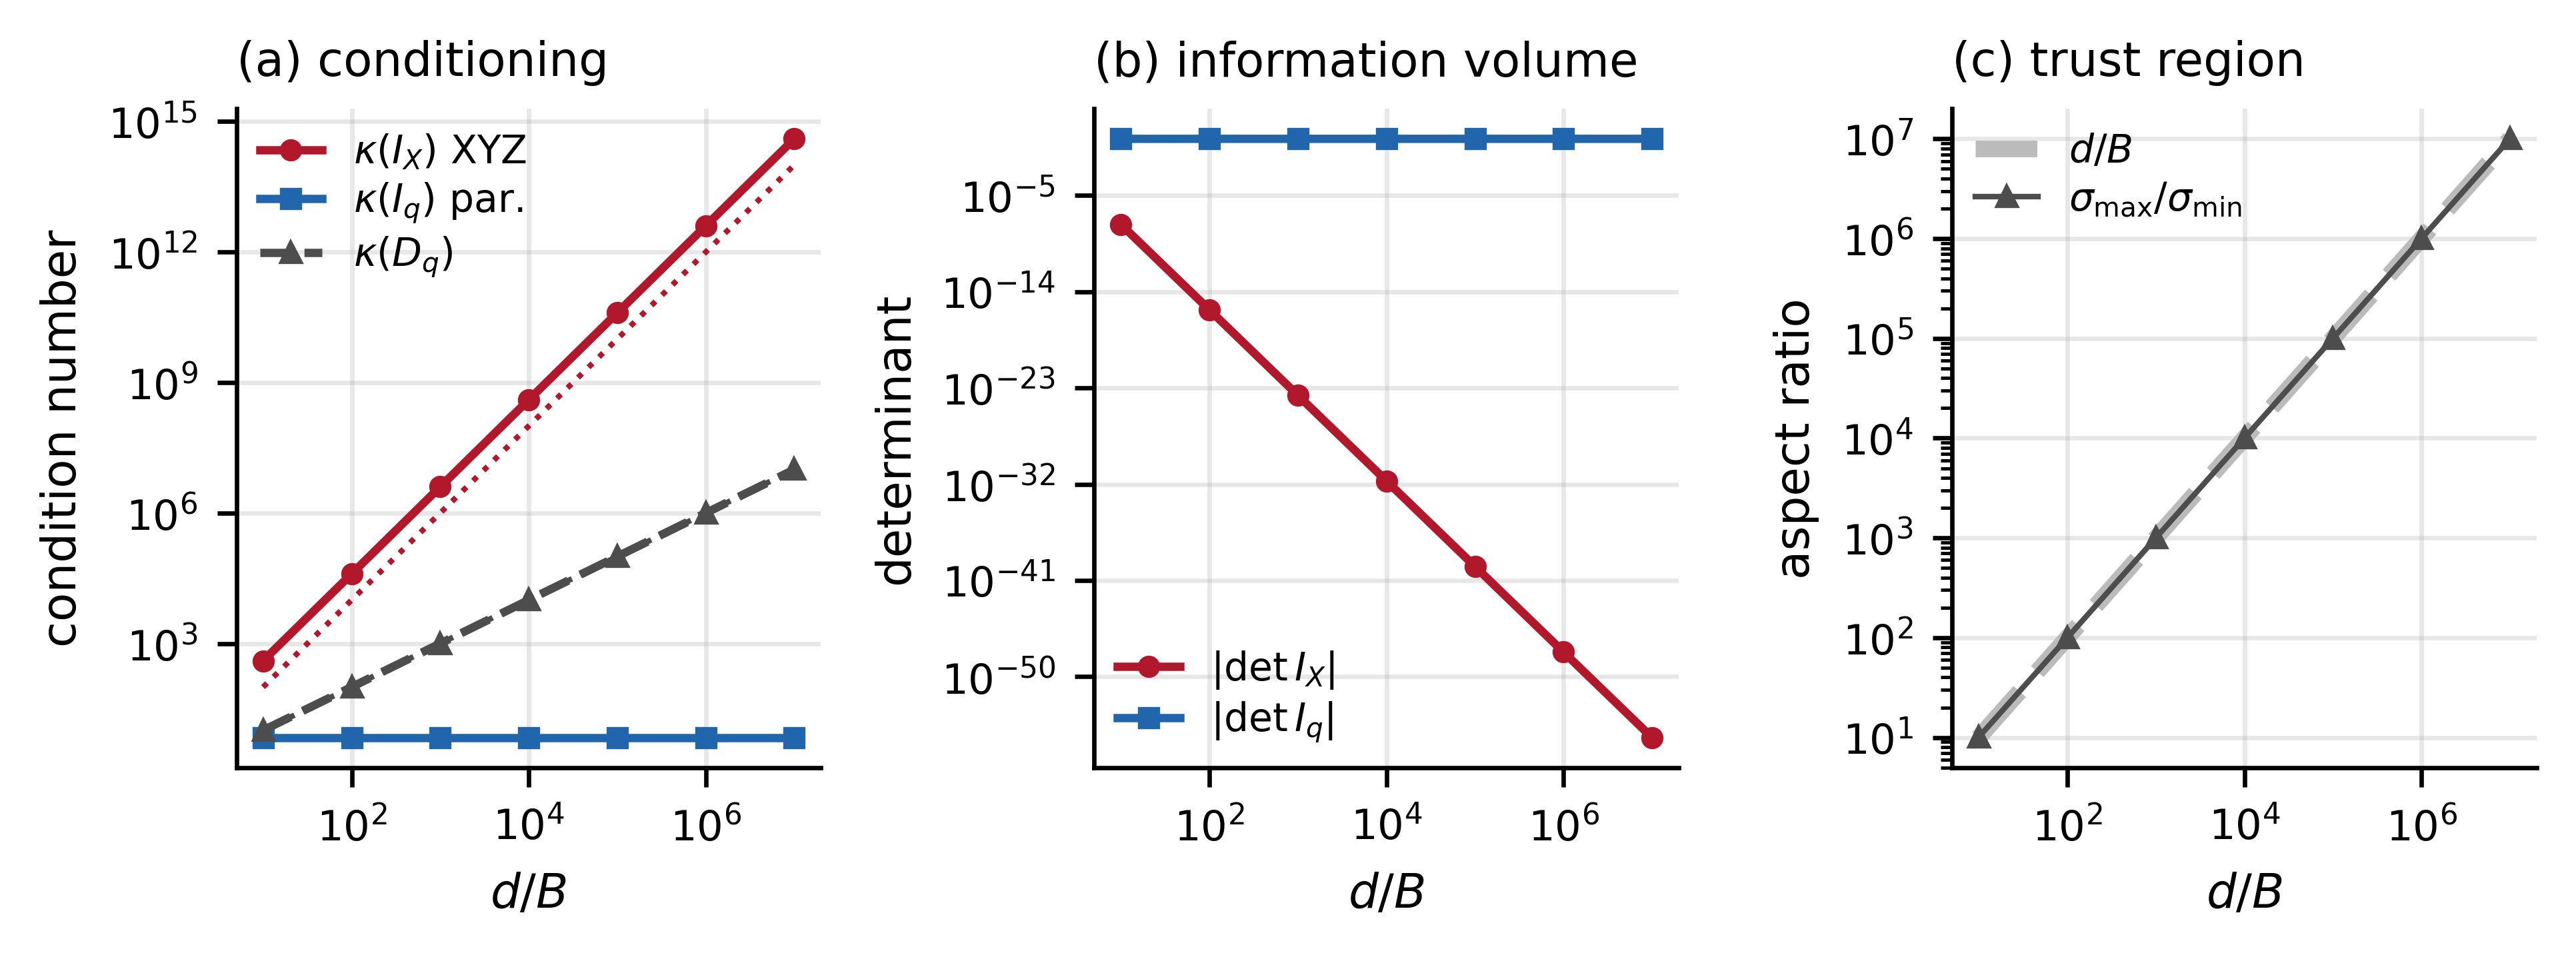
\includegraphics[width=0.97\linewidth]{figures/ba_theorem.png}
\caption{Near-singular asymptotics for $\beta=\pi/2$ and unit baseline, plotted against $d/B=1/\tan\omega$: (a) condition numbers of $I_X$, $I_q$ and $D_q$, with the dotted references $(d/B)^{2}$ and $d/B$; (b) determinants of $I_X$ and $I_q$; (c) aspect ratio of the parallax trust-region ellipsoid against the prediction $d/B$. The condition number of the chart information matrix stays bounded while that of XYZ grows as $(d/B)^{2}$, but the condition number of the chart Jacobian grows as $d/B$, so the improvement is a rescaling of the same physical information.}
\label{fig:ba-asymptotics}
\end{figure}

Figure~\ref{fig:ba-asymptotics} shows the scaling over seven decades. The fitted log--log slopes are $-1.9999$ for $\kappa(I_X)$, $-0.9991$ for $\kappa(D_q)$, $3.9991$ for $n^{\T}I_Xn$, $8.0002$ for $\det I_X$, and $-0.0007$ for $\det I_q$, matching $\kappa(I_X)\sim4\omega^{-2}$, $\kappa(D_q)\sim\omega^{-1}$, $n^{\T}I_Xn\sim\omega^{4}/B^{2}$, $\det I_X\sim2\omega^{8}/B^{6}$ and $\det I_q\to2$. The chart does not create information: $\det I_X$ collapses by eight orders of magnitude per decade of $\omega$ while $\det I_q$ is constant, and the two are related by $\det I_q=(\det D_q)^{2}\det I_X$ with $\det D_q\sim\omega^{-4}$.

On an independent two-view grid, depth and inverse-depth Gauss--Newton steps agree in physical coordinates to $1.10\times10^{-11}$, and pullback-metric Levenberg--Marquardt steps to $9.10\times10^{-13}$.

These asymptotics also locate the original argument. Its $2\times2$ matrix is the two-view instance of $I_q$, and $\det I_q\to2$ is the numerical form of the positive definiteness that the paper reports. Section~\ref{sec:parallaxba} separates what that computation establishes from what has been inferred from it.

\section{What the ParallaxBA Proof Does and Does Not Establish}
\label{sec:parallaxba}

Before Theorem~\ref{thm:main} is applied to it, the original argument is worth stating in its own terms. It is made in a two-view bearing model, and its central computation is a $2\times2$ normal matrix that the paper shows to be positive definite. That computation is correct, and nothing below disputes it. What is at issue is what follows from it: whether it establishes that the chart avoids singularity, whether it establishes that depth remains observable where XYZ and inverse depth lose it, and whether it explains a convergence advantage. The three subsections take these in turn.

\subsection{The two-dimensional matrix is positive definite}
In the simplified two-view bearing model of \citet{zhao2015parallaxba}, the point coordinates are $(\theta,\omega)$ and the predicted bearings are
\begin{equation}
  f_1(\theta,\omega)=\theta-\phi_1,\qquad
  f_2(\theta,\omega)=\theta+\omega-\phi_2.
\end{equation}
Consequently,
\begin{equation}
  J_{\mathrm{pa}}=
  \begin{bmatrix}1&0\\1&1\end{bmatrix},
  \qquad
  J_{\mathrm{pa}}^\T J_{\mathrm{pa}}=
  \begin{bmatrix}2&1\\1&1\end{bmatrix}.
  \label{eq:pa-normal}
\end{equation}
The determinant is one and the matrix is positive definite. This algebraic statement is correct. The original paper also notes that the matrix is no longer constant in three-dimensional BA; Equation~\eqref{eq:pa-normal} should not be misrepresented as a completed general three-dimensional proof.

The relation between the two dimensions is worth stating explicitly, because it is the point at which the original extrapolation fails. The three-dimensional information matrix of the same construction, ordered as $(\beta,\omega,\alpha)$, is
\begin{equation}
I_q=
\begin{bmatrix}
2&1&0\\
1&1&0\\
0&0&S
\end{bmatrix},
\qquad
S=\sin^{2}\beta+\sin^{2}(\beta+\omega),
\label{eq:iq-3d}
\end{equation}
so \eqref{eq:pa-normal} is exactly its $(\beta,\omega)$ block. The third coordinate carries the factor $S$, and $S$ vanishes on the baseline $\beta=\omega=0$ while the $(\beta,\omega)$ block remains positive definite there. The two-dimensional analysis is therefore correct as algebra and incomplete as a reduction: it omits the only coordinate in which three dimensions can degenerate, so its positive definiteness carries no information about the three-dimensional null space.

\subsection{Positive auxiliary rank does not restore depth}
\begin{proposition}[Non-injectivity under aligned motion]
\label{prop:noninjective}
Let the main camera be at the origin, let the associate camera be at $B u_\theta$ with $B>0$, and consider $P=d u_\theta$ for every $d>B$. Both observed rays have direction $u_\theta$, and $\omega=0$ for every such $d$. Hence $(\theta,d)\mapsto(\theta,\omega)$ is neither injective nor a local diffeomorphism on this set.
\end{proposition}
\begin{proof}
The main ray is $P-0=d u_\theta$. The associate ray is $P-Bu_\theta=(d-B)u_\theta$, which has the same direction because $d-B>0$. Their parallax angle is therefore zero independently of $d$. Varying $d$ changes the finite Euclidean point but not the parallax coordinates or the bearings.
\end{proof}

The failure is visible in either chart. Along the aligned family, $\partial\omega/\partial d$ vanishes identically, so the Jacobian of $(\theta,d)\mapsto(\theta,\omega)$ has a zero eigenvalue with eigenvector pointing along $d$. The angular chart hides the same fact in a different form. Depth follows from the sine law of the original appendix \cite{zhao2015parallaxba}, $d=B\sin(\beta+\omega)/\sin\omega$, and its derivative with respect to $\omega$ is $-B\sin\beta/\sin^{2}\omega$. That derivative vanishes at $\beta=0$ and diverges as $\omega\to0$ whenever $\mbox{$\beta\neq0$}$. Depth is therefore either locally insensitive to the parallax angle or catastrophically sensitive to it, and a single formula covers both regimes only because it is evaluated on opposite sides of the alignment. A parameterization that reports a well-conditioned $2\times2$ block for $(\beta,\omega)$ is reporting the conditioning of the angular coordinates, not of $d$.

There is no contradiction between Proposition~\ref{prop:noninjective} and Equation~\eqref{eq:pa-normal}. The matrix establishes that the two angular measurements determine $(\theta,\omega)$ in the auxiliary model. At the aligned configuration, those coordinates do not determine $d$. Indeed, the original paper acknowledges the absence of depth information in this situation. The error would be to use auxiliary rank as evidence of Euclidean depth observability.

The same distinction applies to initialization. In the simplified model,
\begin{equation}
  \omega=(\theta_2+\phi_2)-(\theta_1+\phi_1),
\end{equation}
so the absolute angular error is observation-noise scaled and the angular coordinates start out well conditioned. That is what makes the transfer to depth deceptive rather than visibly ill posed.

\subsection{An exact three-dimensional zero-ray counterexample}
\label{sec:zero-ray}
For a non-main camera $i$, the original ParallaxBA observation function uses the scaled ray \cite[Eq.~(8)]{zhao2015parallaxba}
\begin{equation}
  \tilde x_j^i=
  \sin(\omega_j+\phi_j)\,\|t_a-t_m\|\,x_j^m
  -\sin(\omega_j)(t_i-t_m),
  \label{eq:original-ray}
\end{equation}
where $x_j^m$ is the unit main-anchor bearing and $\phi_j$ is the angle between $t_a-t_m$ and that bearing.

\begin{proposition}[Undefined associate projection at exact collinearity]
\label{prop:zero-ray}
Choose $i=a$, $t_a-t_m=B x_j^m$ with $B>0$, $\phi_j=0$, and $\omega_j=0$. Then Equation~\eqref{eq:original-ray} gives $\tilde x_j^a=0$. A perspective projection $x/z,\ y/z$ is undefined at this zero vector.
\end{proposition}
\begin{proof}
Direct substitution yields
\begin{equation}
  \tilde x_j^a=\sin(0)\,B x_j^m-\sin(0)\,B x_j^m=0.
\end{equation}
Both image ratios require division by the third coordinate of this zero vector.
\end{proof}

This is not merely an arbitrary inconsistent choice of angles. As in Proposition~\ref{prop:noninjective}, every finite point $P=d x_j^m$ with $d>B$ realizes the same aligned, zero-parallax geometry. The degenerate set is therefore physically meaningful, even if exact equality has probability zero under an absolutely continuous noise model.

Appendix A of Zhao et al. derives the depth using
\begin{equation}
  d_j=\frac{\sin(\omega_j+\phi_j)}{\sin\omega_j}\|t_a-t_m\|,
  \label{eq:sine-law}
\end{equation}
and then multiplies the ray by $\sin\omega_j$ to avoid the denominator. This scaling preserves homogeneous projection when the underlying finite ray exists and the scale is nonzero. At zero parallax, however, the division in Equation~\eqref{eq:sine-law} is already singular and the scaled ray can collapse to zero. Removing a denominator algebraically is not proof that the geometric singularity has been removed.

This counterexample does not show that ParallaxBA always diverges, that every implementation evaluates the same expression without guards, or that PMBA inherits the same domain. It does falsify an unconditional reading of the claim that the original three-dimensional observation model has no issue for such near-zero-parallax features. Theorem~\ref{thm:main} has already settled the corresponding question for the full normal equations: at this configuration the reduced camera system loses one physical direction for every chart at once, so the zero ray is a property of the geometry that the chart was meant to repair.

These claims were checked with deterministic standard-library scripts. The aligned example reproduces Equation~\eqref{eq:pa-normal}, the depth-to-parallax derivative has zero second row, and the three-dimensional substitution returns a zero ray and an undefined projection. For an aligned angle separation $\phi=0.01$ and depth $d=100$, the unscaled point-block condition numbers are approximately $3.92\times10^{12}$ for depth and $3.92\times10^{4}$ for inverse depth; after diagonal column normalization, both correlation-matrix condition numbers are $5.9121$. Raw condition numbers therefore separate two charts that the normalized problem does not, which is the scalar form of the argument of Section~\ref{sec:ba-theorem}. It does not predict the full Schur system of a production solver, and it does not pre-empt the controlled study of Section~\ref{sec:synthetic}.

\subsection{What implementations do instead}
\label{sec:cep}
No implementation evaluates \eqref{eq:original-ray} unguarded, and the guard is worth naming, because it is what makes the degeneracy invisible in practice. A Ceres-based implementation of the method replaces the triangulation factor by
\begin{equation}
  \widehat{s}_\beta=
  \sqrt{\max(0,1-\cos^2\beta)+\epsilon^2},\qquad \epsilon=10^{-12},
  \label{eq:cep-floor}
\end{equation}
and floors the baseline norm in the same way. At $\beta=\omega=0$ in the associate view this produces a small nonzero ray and a finite automatic-differentiation value: a numerical continuation of a degenerate expression, not a consequence of the original proof.

It is not even the continuation of the nearby limit. In a planar associate-view model with main bearing $u(\beta)=(\cos\beta,\sin\beta)$ and baseline direction $(1,0)$, Equation~\eqref{eq:original-ray} reduces, up to the positive baseline scale, to
\begin{equation}
  v(\beta,\omega)=
  \begin{bmatrix}
  \sin(\beta+\omega)\cos\beta-\sin\omega\\
  \sin(\beta+\omega)\sin\beta
  \end{bmatrix}.
  \label{eq:reduced-ray}
\end{equation}
For fixed $\omega$ one has $\lim_{\beta\to0^+}v(\beta,\omega)/\beta=(\cos\omega,\sin\omega)^\T$, a ray of bearing $\omega$. But $v(0,\omega)=0$, while the floor returns $v_\epsilon(0,\omega)=(\epsilon\cos\omega,0)^\T$, a ray of bearing zero. An $\epsilon$ therefore supplies a value where the model has none, and supplies the wrong one. The same expression computes $1-\cos^2\beta$ in floating point, which can round to zero before the floor is applied, so the guard is not uniform in $\beta$ either.

The consequence is procedural rather than damning. A robustness claim should name the regularized residual it actually minimises and report the ray norm, $\sin\omega$, behind-camera states and anchor geometry, because a floor that prevents NaNs is not by itself evidence of uniform conditioning.

\section{A Normalized Complementary Parallax Chart}
\label{sec:normalized-chart}
The zero-ray counterexample motivates a domain question rather than an immediate claim that another coordinate will converge faster. We keep the notation of Section~\ref{sec:chart-family} but now hold the anchors fixed, so that the chart is an ordinary change of variables. Let $C_m$ and $C_a$ be fixed main and associate anchor centres, $b=C_a-C_m$, $B=\|b\|>0$, and let $n$ be the unit main-anchor bearing. Write $\beta$ for the angle between $n$ and $b$. On the original chart's regular domain, sine-law triangulation gives the Euclidean reconstruction
\begin{equation}
  d=n^\T b+B\sin\beta\cot\omega,
  \qquad X=C_m+d\,n .
  \label{eq:raw-depth}
\end{equation}
Define the normalized scalar coordinate
\begin{equation}
  \boxed{\nu=\frac{\tan\omega}{\sin\beta}} .
  \label{eq:normalized-coordinate}
\end{equation}
On the common domain, $n^\T(X-C_a)=B\sin\beta\cot\omega$, and therefore
\begin{equation}
  \nu=\frac{B}{n^\T(X-C_a)},
  \qquad
  \boxed{X=C_m+\left(n^\T b+\frac{B}{\nu}\right)n} .
  \label{eq:normalized-reconstruction}
\end{equation}
Thus $\nu$ is an inverse-depth-like coordinate measured along the main bearing relative to the associate anchor. Equation~\eqref{eq:normalized-reconstruction} requires neither an inverse sine nor the original scaled ray.

\begin{proposition}[Exact common-domain equivalence and aligned coverage]
\label{prop:normalized-chart}
Where both charts are regular, Equations~\eqref{eq:raw-depth} and \eqref{eq:normalized-reconstruction} represent the same physical point and the same reprojection objective. Moreover, for aligned anchors $b=Bn$ and any finite point $X=C_m+dn$ with $d>B>0$, the normalized coordinate $\nu=B/(d-B)$ is finite and reconstructs $X$, although the original parallax angle is $\omega=0$ and Equation~\eqref{eq:original-ray} collapses to the zero ray in the associate view.
\end{proposition}
\begin{proof}
The common-domain identities follow by substituting $\cot\omega=1/(\nu\sin\beta)$ into Equation~\eqref{eq:raw-depth}. In the aligned case, $n^\T(X-C_a)=d-B$, so $B/\nu=d-B$ and $n^\T b+B/\nu=d$. Proposition~\ref{prop:zero-ray} gives the original zero-ray statement.
\end{proof}

The distinction is also visible in the coordinate Jacobians. At fixed anchors, use an orthonormal tangent basis for the two bearing coordinates. The determinants of the maps from chart coordinates to Euclidean point coordinates are
\begin{align}
  |\det D_{\mathrm{raw}}|
    &=d^2B\,\frac{|\sin\beta|}{\sin^2\omega},\\
  |\det D_{\mathrm{norm}}|
    &=\frac{d^2B}{\nu^2} .
  \label{eq:chart-determinants}
\end{align}
The raw determinant explicitly vanishes with $\sin\beta$ or $\sin\omega$; the normalized determinant has no $\sin\beta$ factor. This establishes a complementary domain, not a globally regular atlas: $\nu=0$, $\nu\to\infty$, $B=0$, and $d=0$ remain boundaries or singular limits. Nor does Equation~\eqref{eq:normalized-reconstruction} add an observation or restore depth information when the physical rays are identical. In particular, a nonsingular $D_{\mathrm{norm}}$ cannot make $J_xD_{\mathrm{norm}}$ full rank when the physical measurement Jacobian $J_x$ is itself rank deficient.

\subsection{What the repair does not buy}
For $x=g(q)$ and $F=\tfrac12\|r\|^2$, the full Hessian in $q$ is
\begin{equation}
  \nabla_q^2F
  =D^\T\nabla_x^2F\,D
  +\sum_{\ell}\frac{\partial F}{\partial x_\ell}\,\nabla_q^2g_\ell .
  \label{eq:full-hessian}
\end{equation}
Away from a stationary point, the gradient-weighted coordinate-curvature term need not vanish. The GN matrix retains only first-order residual derivatives, and Theorem~\ref{thm:gn} establishes equality of one local physical step, not equality of damped or nonlinear finite-budget trajectories. Consequently, neither a smaller raw condition number nor a larger one-step predicted decrease is by itself a theorem about eventual convergence. Any proposed chart selector must be tested against complete paired trajectories.

The normalized-chart identities were checked on 159 positive-depth common-domain cases: the largest physical-point discrepancy was $2.18\times10^{-15}$ and the largest transition-coordinate discrepancy $6.82\times10^{-13}$. On 119 moderately scaled finite-difference cases, the largest relative errors of the raw and normalized determinant formulas of \eqref{eq:chart-determinants} were $2.24\times10^{-9}$ and $1.98\times10^{-9}$. Separate aligned examples with $d=1.5,4,100$ reconstruct finite points in the normalized chart while the original scaled ray is zero. These checks validate the algebra and the implementation identities, not a convergence advantage.

\section{Controlled Synthetic Validation}
\label{sec:synthetic}

\subsection{Why a synthetic study}
The results of Sections~\ref{sec:framework}--\ref{sec:ba-theorem} make predictions that are quantitative and therefore falsifiable: on a regular chart the physical Gauss--Newton step and the Fisher information are invariant, the chart Hessian condition number is not, the damping metric is the only free object, and every chart loses the same physical rank at a degenerate configuration. Deciding whether these predictions hold requires a scene whose ground truth is known, because the decisive quantity is the error of the estimated depth, not the reprojection residual.

We deliberately do not use a benchmark corpus in this section. A corpus confounds the chart with the initialization, the solver settings, and the iteration budget, and its scenes are not a random sample of any population, so instance-level success counts cannot be read as estimates of a success probability. More importantly, the usual success criterion is a threshold on final reprojection error, and Section~\ref{sec:depth-blind} shows that this criterion is nearly blind to depth error in exactly the regime where charts are supposed to differ. The questions here are mechanism questions; they are better answered where the answer is measurable.

\subsection{Protocol}
Each scene contains six cameras on a straight forward-moving rig with $0.4$\,m spacing and a pinhole model of unit focal length. Twenty background points are drawn in front of the last camera, and one \emph{probe} point is placed at $12$\,m on a cone of controlled half-angle $\beta$ about the motion axis. Image coordinates carry independent Gaussian noise with standard deviation $10^{-3}$, corresponding to $0.5$\,px at $f=500$.

Bearing-only BA has a seven-dimensional gauge group: six rigid-body degrees of freedom and one global scale. We fix camera~0 completely and fix the baseline of camera~1, which removes all seven. Without the scale constraint every Hessian below would be rank deficient by one for a reason unrelated to the chart, and no rank comparison would be meaningful.

Four charts are compared: global XYZ; optical-axis inverse depth $(u,v,\rho)$ anchored at camera~0~\cite{civera2008inverse}; inverse Euclidean range with a world bearing; and the parallax chart of \eqref{eq:chart} anchored at camera~0 and the last camera, that is, on the longest available baseline. Every chart is initialized from the \emph{same} perturbed physical point cloud by exact inversion of its own chart map, so the initial reprojection cost is common by construction. All solves use one Schur-complement LM implementation, one stopping rule, and, unless stated otherwise, an isotropic $\lambda I$ with $\lambda_0=10^{-4}$ under the schedule of Section~\ref{sec:damping}. No timing is reported, and no claim is made about global optimality.

\subsection{The chart cannot change the Gauss--Newton iterates}
Table~\ref{tab:gn-invariance} runs undamped Gauss--Newton from a shared initialization on a regular sideways rig with a transverse baseline, where $\beta\approx\pi/2$ and no chart is near a singular locus.

\begin{table}[t]
\centering
\caption{Undamped Gauss--Newton from one shared physical initialization on a regular six-camera problem (24 points, 144 observations). Every chart reaches the same physical solution. The last column compares the reconstructed point cloud with the XYZ result.}
\label{tab:gn-invariance}
\small
\setlength{\tabcolsep}{4.2pt}
\begin{tabular}{llrrrr}
\toprule
Chart & Point parameters & Iter. & Final cost & Depth error & Position difference\\
\midrule
XYZ & $(X,Y,Z)$ & 4 & $2.2\times10^{-31}$ & $1.5\times10^{-15}$ & ---\\
Inverse depth & $(u,v,\rho)$ & 1 & $8.6\times10^{-31}$ & $6.3\times10^{-15}$ & $3.7\times10^{-14}$\,m\\
Inverse range & $(\theta,\phi,\rho)$ & 4 & $5.9\times10^{-31}$ & $8.8\times10^{-16}$ & $3.7\times10^{-14}$\,m\\
Parallax & $(\alpha,\beta,\omega)$ & 4 & $1.2\times10^{-30}$ & $8.7\times10^{-16}$ & $3.7\times10^{-14}$\,m\\
\bottomrule
\end{tabular}
\end{table}

The largest position difference between any two charts is $3.7\times10^{-14}$\,m, and every chart recovers the depth to $10^{-15}$. This is not an empirical coincidence but Theorem~\ref{thm:gn} applied iteratively, and it holds because the problem is regular. The consequence for the original argument is immediate. A statement of the form ``ParallaxBA converges where XYZ or inverse depth diverges'' cannot be a statement about information or about the Gauss--Newton map: on a regular problem the iterates are the same sequence written in different coordinates. Such a difference can arise only from a singular linear solve, from damping, or from the domain. Sections~\ref{sec:sweep}--\ref{sec:damping-sec} examine each of the three.

\subsection{Conditioning is not uncertainty}
\label{sec:sweep}
Table~\ref{tab:sweep} sweeps the probe from $80^\circ$ down to $0.1^\circ$ of the motion axis and reports, at the true configuration, the condition number of each chart Hessian and the marginal standard deviation of the probe depth from the Cram\'er--Rao bound \cite{kay1993estimation}.

\begin{table}[!tb]
\centering
\caption{Angle sweep at fixed depth ($12$\,m) and noise ($\sigma=10^{-3}$). Columns 2--5 are condition numbers of the chart Hessian at the true configuration. Column 6 is the marginal standard deviation of the probe depth; it agrees across the four charts to a maximum relative spread of $2.8\times10^{-10}$, so one column is shown. Columns 7--8 are the parallax parameter standard deviation and $|\partial d/\partial\omega|$.}
\label{tab:sweep}
\small
\begin{tabular}{lrrrrrrr}
\toprule
$\beta$ & $\kappa(H)$ XYZ & $\kappa(H)$ ID & $\kappa(H)$ IR & $\kappa(H)$ PA & $\sigma_d$ (m) & $\sigma_\omega$ (rad) & $|\partial d/\partial\omega|$\\
\midrule
$80^\circ$ & $5.3\times10^{10}$ & $3.5\times10^{7}$ & $1.3\times10^{8}$ & $2.3\times10^{8}$ & $8.96\times10^{-2}$ & $1.27\times10^{-3}$ & $71$\\
$45^\circ$ & $2.2\times10^{8}$ & $1.4\times10^{5}$ & $2.8\times10^{5}$ & $6.9\times10^{5}$ & $1.14\times10^{-1}$ & $1.65\times10^{-3}$ & $81$\\
$20^\circ$ & $2.2\times10^{8}$ & $1.3\times10^{5}$ & $2.7\times10^{5}$ & $6.9\times10^{5}$ & $2.28\times10^{-1}$ & $1.84\times10^{-3}$ & $150$\\
$8^\circ$ & $3.7\times10^{8}$ & $1.4\times10^{5}$ & $2.8\times10^{5}$ & $9.8\times10^{5}$ & $5.74\times10^{-1}$ & $1.92\times10^{-3}$ & $360$\\
$3^\circ$ & $2.0\times10^{9}$ & $1.8\times10^{5}$ & $4.1\times10^{5}$ & $4.1\times10^{6}$ & $1.53$ & $1.94\times10^{-3}$ & $960$\\
$1^\circ$ & $1.8\times10^{10}$ & $1.0\times10^{6}$ & $2.5\times10^{6}$ & $3.4\times10^{7}$ & $4.60$ & $1.94\times10^{-3}$ & $2900$\\
$0.3^\circ$ & $2.0\times10^{11}$ & $1.1\times10^{7}$ & $2.7\times10^{7}$ & $3.7\times10^{8}$ & $15.3$ & $1.94\times10^{-3}$ & $9500$\\
$0.1^\circ$ & $1.8\times10^{12}$ & $9.9\times10^{7}$ & $2.4\times10^{8}$ & $3.4\times10^{9}$ & $46.0$ & $1.94\times10^{-3}$ & $29000$\\
\bottomrule
\end{tabular}
\end{table}

Three features of Table~\ref{tab:sweep} and Figure~\ref{fig:synthetic} matter. First, the condition numbers range over seven orders of magnitude, from $1.3\times10^{5}$ to $1.8\times10^{12}$, while $\sigma_d$ is a single curve: the four charts agree to a relative difference below $3\times10^{-10}$ at every angle. Conditioning measures the shape of a coordinate ellipsoid, not the information it carries. This is Hartley's normalization in another guise: rescaling the data changes the condition number a solver reports without changing the estimate it obtains \cite{hartley1997eightpoint}. Second, the small and nearly constant $\sigma_\omega$ is compensated by $|\partial d/\partial\omega|$, which grows by the same factor of about $500$; to within the twenty percent contributed by the $\beta$ direction and its correlations, $\sigma_d=\sigma_\omega|\partial d/\partial\omega|$. This is the chain rule of Theorem~\ref{thm:gn} in probabilistic form. The parallax chart has a well-conditioned angle because it has chosen to measure a well-conditioned quantity; the ill-conditioning has moved into the map from that quantity to depth, where it is no longer visible in $\kappa(H)$.

Third, and contrary to the premise of the original comparison, inverse depth has the \emph{smallest} condition number of the four charts at every angle in this scene. The parallax chart is better conditioned than XYZ by one to two orders of magnitude, but it is worse conditioned than inverse depth by a factor of two to forty. Whatever a conditioning argument can support, it cannot support a general claim that parallax coordinates are better conditioned than inverse-depth coordinates.

\begin{figure}[t]
\centering
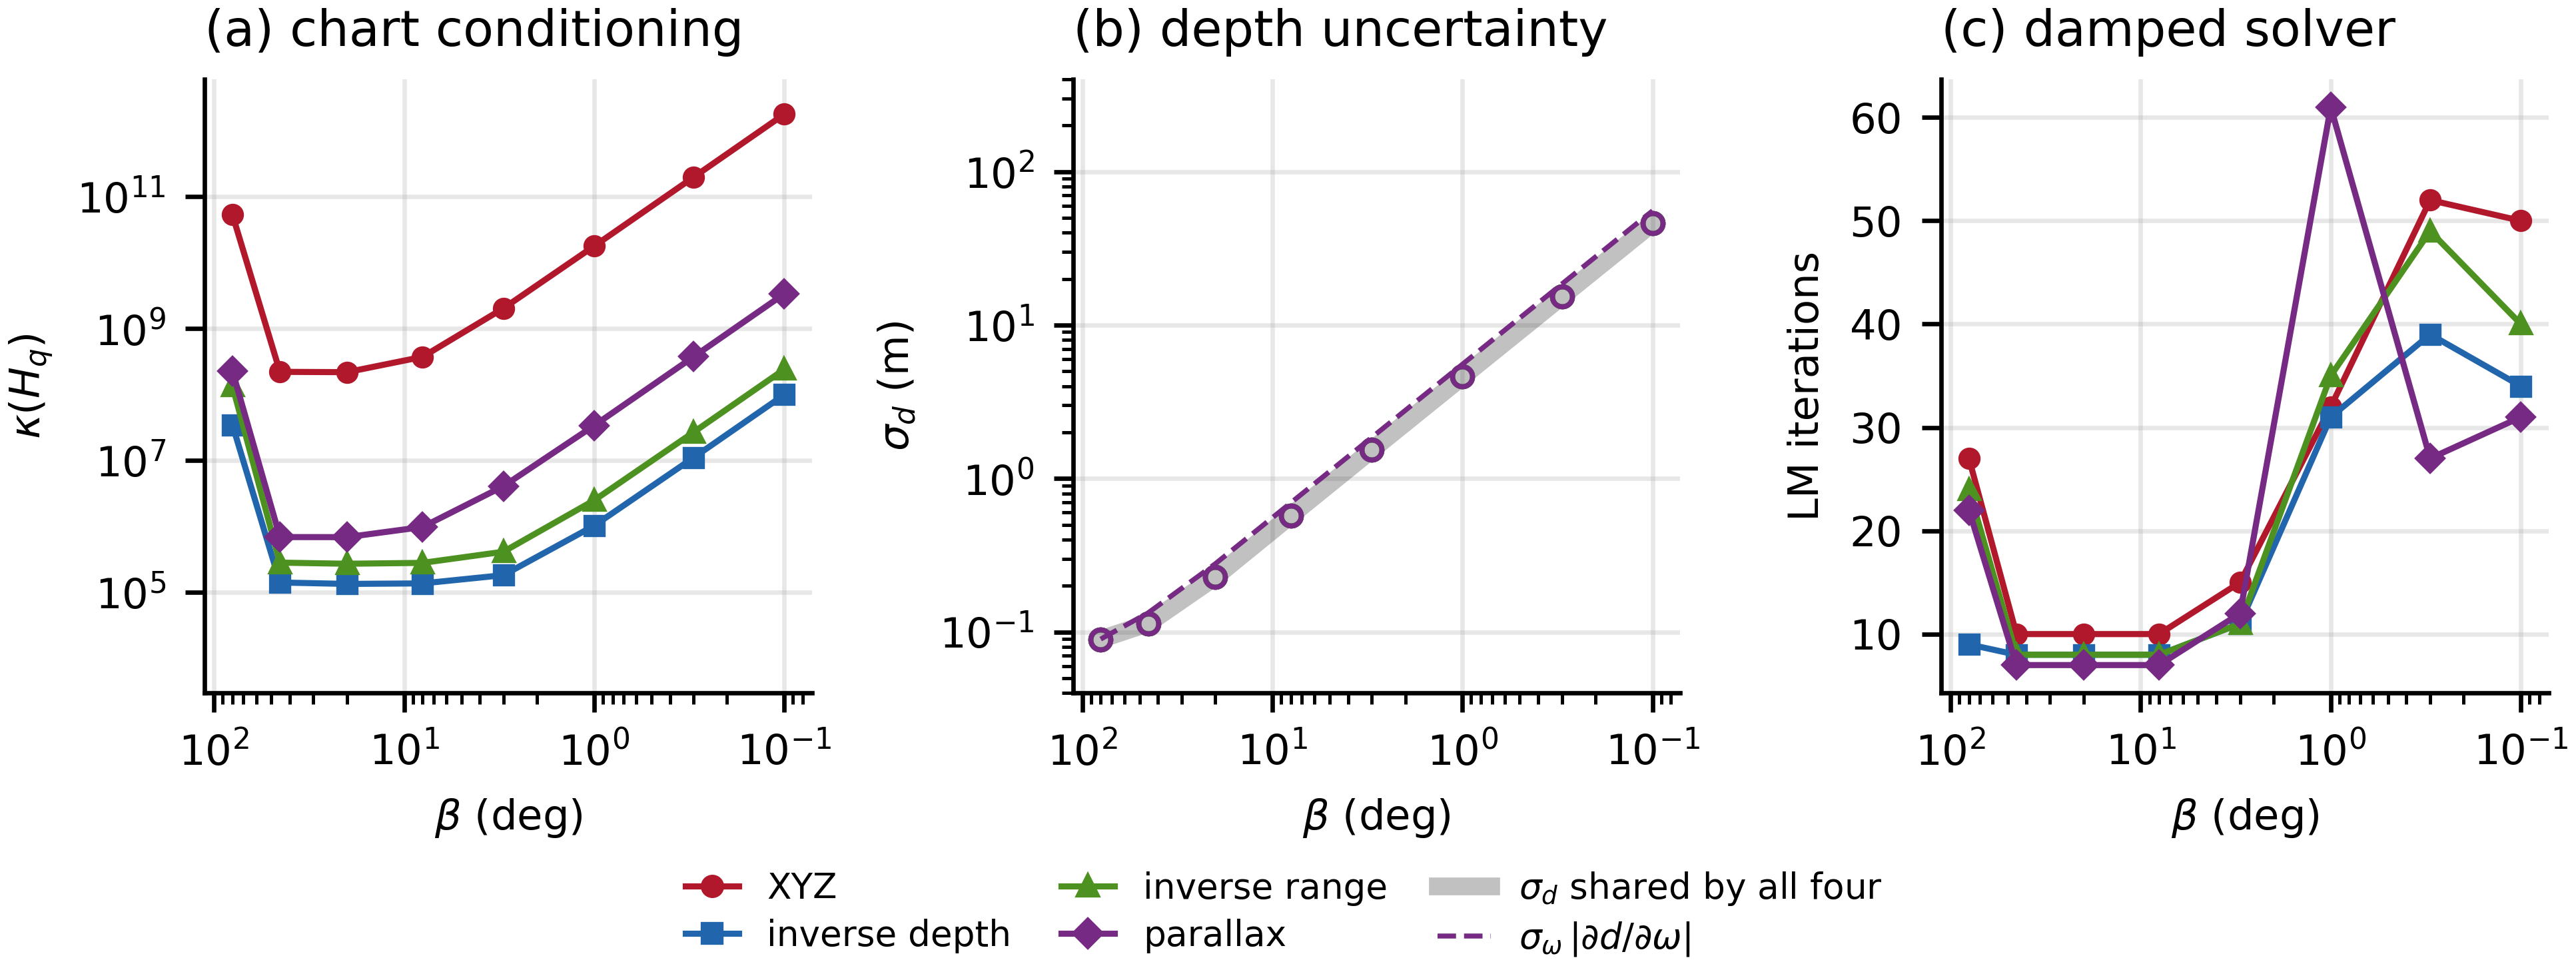
\includegraphics[width=0.96\linewidth]{figures/synthetic_chart.png}
\caption{Controlled angle sweep. (a) Condition number of the chart Hessian at the true configuration: the four charts span three orders of magnitude at a fixed angle and seven across the sweep, and the XYZ curve grows as $\omega^{-2}$. (b) Marginal depth standard deviation from the Cram\'er--Rao bound. The four charts coincide to a relative difference below $3\times10^{-10}$; the dashed curve is $\sigma_\omega|\partial d/\partial\omega|$. (c) Iterations of the same damped solver from a shared initialization. Iteration counts differ by up to a factor of three in either direction with no consistent ordering.}
\label{fig:synthetic}
\end{figure}

\subsection{At exact alignment every chart loses the same rank}
\label{sec:alignment}
We place the probe exactly on the motion axis and evaluate every Hessian at the true configuration. XYZ and inverse depth each give $\operatorname{nullity}H=1$, with a direct Gauss--Newton solve that fails on a singular matrix. Inverse range gives $\operatorname{nullity}H=2$ and a direct solve that succeeds. In all three cases the reduced camera matrix keeps full rank, $\operatorname{nullity}\mathcal S=0$. The parallax chart is undefined, because $\sin\omega=0$ at $\beta=0$.

The physical rank loss is one: the probe's distance is not observed. XYZ and inverse depth exhibit exactly that direction. Inverse range exhibits an extra one because the probe lies on the pole of its spherical bearing chart; by Corollary~\ref{cor:fates} this is a chart pseudo-null direction, which adds one to the nullity of $H$ without removing anything from the reduced system. And the parallax chart cannot represent the configuration at all: at $\beta=0$ the map \eqref{eq:chart} is $0/0$, so there is no Jacobian to evaluate and no positive-definite matrix to report.

These are three different answers to what is physically the same rank-one deficiency. Which chart reports a singular normal-equation system is a property of the chart, not of the problem, and a solver log that records one is recording a coordinate artifact rather than a failure of the observation model.

\subsection{Damping, not information}
\label{sec:damping-sec}
Table~\ref{tab:damping} takes one damped step from the shared initialization at $\beta=1^\circ$ and compares, on the left, the effect of using the same numerical $\lambda$ in every chart and, on the right, the effect of holding the physical damping ellipsoid fixed through the pullback metric $\lambda T^{-\top}T^{-1}$ of Theorem~\ref{thm:damping}.

\begin{table}[t]
\centering
\caption{One damped step from a shared initialization at $\beta=1^\circ$. Entries are relative differences from the XYZ step. Left: the same $\lambda$ in every chart, which is the usual comparison. Right: $\lambda$ interpreted through the physical metric $T^{-\top}T^{-1}$, so that the damping ellipsoid is chart invariant.}
\label{tab:damping}
\small
\begin{tabular}{lrrrrrr}
\toprule
& \multicolumn{3}{c}{same $\lambda$ in every chart} & \multicolumn{3}{c}{pulled-back metric}\\
\cmidrule(lr){2-4}\cmidrule(lr){5-7}
$\lambda$ & ID & IR & PA & ID & IR & PA\\
\midrule
$10^{-8}$ & $1.0\times10^{-3}$ & $1.0\times10^{-3}$ & $1.0\times10^{-3}$ & $2.5\times10^{-11}$ & $2.0\times10^{-11}$ & $9.3\times10^{-12}$\\
$10^{-6}$ & $7.5\times10^{-2}$ & $7.5\times10^{-2}$ & $7.4\times10^{-2}$ & $1.4\times10^{-11}$ & $1.8\times10^{-11}$ & $2.3\times10^{-11}$\\
$10^{-4}$ & $5.9\times10^{-1}$ & $6.0\times10^{-1}$ & $5.0\times10^{-1}$ & $5.2\times10^{-12}$ & $1.1\times10^{-11}$ & $2.2\times10^{-12}$\\
$10^{-2}$ & $7.8\times10^{-1}$ & $1.27$ & $8.6\times10^{-1}$ & $1.6\times10^{-11}$ & $2.2\times10^{-12}$ & $9.7\times10^{-12}$\\
$10^{0}$ & $4.15$ & $3.00$ & $4.88$ & $2.6\times10^{-13}$ & $6.0\times10^{-13}$ & $4.7\times10^{-13}$\\
\bottomrule
\end{tabular}
\end{table}

With a shared $\lambda$ the chart steps depart from the XYZ step by relative differences ranging from $10^{-3}$ at $\lambda=10^{-8}$ to $4.9$ at $\lambda=10^{0}$, where the parallax step is $5.2$ times longer than the XYZ step in norm. The limit $\lambda\to0$ is a second, independent confirmation of Theorem~\ref{thm:gn}: at $\lambda=10^{-8}$ the four step norms are $4.2843$, $4.2861$, $4.2861$ and $4.2861$, a spread of $4\times10^{-4}$. The ranking of the charts also changes with $\lambda$: at $10^{-4}$ parallax is closest to XYZ, at $10^{-2}$ inverse depth is, and at $10^{0}$ inverse range is. With the pulled-back metric every chart reproduces the physical reference to $1.1\times10^{-11}$ or better at every $\lambda$. A damped trajectory is therefore a property of the pair $(\text{chart},\lambda)$, not of the chart alone. Iteration counts collected at a single nominal $\lambda$ measure the unit system in which $\lambda$ is expressed, which is why the smooth iteration curves of Figure~\ref{fig:synthetic}(c) carry no ordering that survives a change of damping rule.

\subsection{What a reprojection criterion can see}
\label{sec:depth-blind}
The remaining question is whether the usual success criterion could have decided the issue. Table~\ref{tab:depth-blind} scales the probe's depth from its true value at a fixed bearing and records the change in reprojection error.

\begin{table}[t]
\centering
\caption{Reprojection RMSE produced by a pure depth error, at the same bearing, for a five-camera baseline of $2$\,m and a depth of $12$\,m. The measurement noise used throughout this section is $0.5$\,px.}
\label{tab:depth-blind}
\small
\begin{tabular}{lrrrr}
\toprule
Depth ratio & $\beta=3^\circ$ & $\beta=1^\circ$ & $\beta=0.3^\circ$ & $\beta=0.1^\circ$\\
\midrule
$\times2$ & $1.65$ & $0.55$ & $0.165$ & $0.055$\\
$\times5$ & $2.53$ & $0.84$ & $0.252$ & $0.084$\\
\bottomrule
\end{tabular}
\end{table}

At $\beta=1^\circ$ a fivefold depth error changes the reprojection RMSE by $0.84$\,px, and at $\beta=0.3^\circ$ by $0.25$\,px, which is half the noise. Below about half a degree, a criterion based on final reprojection error, or on a percentage of the best observed error, cannot distinguish a fivefold depth error from measurement noise. It follows that a success count on such a criterion is not evidence about depth accuracy in the regime where the charts are supposed to differ, however the corpus is assembled.

The sweep contains a direct instance of the failure. At $\beta=1^\circ$ the parallax chart returns \texttt{converged} after 61 iterations with a reprojection RMSE of $0.396$\,px, while its relative depth error is $1.5\times10^{11}$; the other three charts stop at $0.298$ on the same problem. The solver declared success on a run whose probe had been pushed to infinity, because the cost it was minimizing is flat in that direction at the available precision. A reported convergence therefore identifies the chart in which the solver gave up, not the geometry it recovered.

\subsection{Reinterpreting the three original observations}
The three observations that motivated ParallaxBA now have explanations that do not require a difference in information.

\emph{Gauss--Newton divergence.} At alignment the normal-equation matrix is singular in every chart, because the probe's depth is unobserved. XYZ and inverse depth return a singular matrix; inverse range returns a matrix with an extra chart pseudo-null direction; the parallax chart is undefined. Which solver log records a failure is decided by the chart, not by the problem.

\emph{The flat objective function.} The objective is a function of the physical point and is therefore chart invariant. What differs is the axis along which it is plotted. At $\beta=1^\circ$ the parallax coordinate has $\sigma_\omega=1.9\times10^{-3}$\,rad while the depth has $\sigma_d=4.6$\,m; the profile in $\omega$ is well curved and the profile in $d$ is flat, and the ratio between the two curvatures is $(\partial d/\partial\omega)^{2}\approx8\times10^{6}$. A one-dimensional plot along $\omega$ therefore shows a well-conditioned objective for a parameter that, at alignment, does not move the point at all.

\emph{Fewer iterations.} With the damping metric held fixed, all charts produce the same step (Table~\ref{tab:damping}); with a shared nominal $\lambda$, the iteration counts differ by up to a factor of three in either direction and reorder when $\lambda$ changes (Figure~\ref{fig:synthetic}(c)). Down to $\beta=3^\circ$ all four converge, and they reach the same depth error and the same reprojection RMSE to four significant digits, for example $0.0648$ and $0.3792$\,px at $\beta=3^\circ$; the attainable minimum is a property of the problem, and only the path to it depends on the chart. Neither behaviour is an information advantage.

What survives is what Theorem~\ref{thm:main} leaves free: the chart Hessian condition number, which is a preconditioning property, and the domain, which decides whether a configuration can be represented at all. Both are real. Neither is a statement about depth observability, and neither distinguishes parallax from inverse depth in a way that is stable across scenes: in Table~\ref{tab:sweep} inverse depth is the better-conditioned of the two at every angle.

\section{Re-running Simulation~2 with the Control It Omits}
\label{sec:repro}
Section~6.1.2 of the original is the experiment aimed directly at inverse depth, and it is the one an author would cite against our account. We therefore rebuilt it, and we report what happened when the missing case was run.

\subsection{The experiment that is cited, and the case it does not run}
Table~3 of the original is a two-pair design. Simulation~1 compares ParallaxBA against XYZ; Simulation~2 compares ParallaxBA against inverse depth. \emph{XYZ is never run on Simulation~2.} The scene is defined by features lying along the direction of camera motion, which is a statement about the geometry and not about a point coordinate. The comparison that would separate ``inverse depth is singular'' from ``that geometry is singular'' is exactly the Euclidean row, and it is absent. Everything below supplies it.

\subsection{Protocol}
We use the sensor of Table~1 (focal $400$\,px, $800\times800$, principal point at the centre, $\pm45^\circ$ field of view, image noise $\sigma=0.1$\,px) and the trajectory of Table~2 ($21$ poses, $2$\,m per step, straight line). The feature box of the original spans only $10$\,m in depth, so with a $40$\,m traverse most of its points fall behind the last camera; we place $120$ features in a slab $45$--$75$\,m ahead instead, of which $24$ lie within $0.6$--$5$\,m of the optical axis. The angle $\beta$ between a feature bearing and the motion axis has median $19.5^\circ$, median $2.3^\circ$ over the near-axis subset, and minimum $0.57^\circ$; the near-degeneracy the original describes is present.

All four charts start from one physical state, obtained by two-view triangulation of each feature's widest observed pair with a cheirality check. The median initial depth error is $4.7\times10^{-4}$ and the near-axis median is $3.2\times10^{-3}$, so the initialization is neither privileged nor sabotaged. The gauge is fixed as in Section~\ref{sec:synthetic}.

\subsection{The conditioning is chart-dependent; the system being solved is not}
\begin{table}[t]
\centering
\caption{Conditioning at the true configuration on the Simulation~2 geometry. $\kappa(H)$ is the quantity the original plots in its Figure~7(b); $\kappa(\mathcal S)$ is the reduced camera system that a Schur-based solver actually factorizes. The first varies by a factor of $366$ across charts, the second by $3\times10^{-9}$.}
\label{tab:repro-cond}
\small
\begin{tabular}{lrrrr}
\toprule
Chart & $\kappa(H)$ & $\kappa(H_{pp})$ & $\kappa(\mathcal S)$ & $\operatorname{rank}\mathcal S$\\
\midrule
XYZ & $7.73\times10^{9}$ & $9.48\times10^{5}$ & $1.628\,171\times10^{8}$ & $117$\\
Inverse depth & $6.82\times10^{10}$ & $2.72\times10^{4}$ & $1.628\,171\times10^{8}$ & $117$\\
Inverse range & $7.02\times10^{10}$ & $1.69\times10^{7}$ & $1.628\,171\times10^{8}$ & $117$\\
Parallax & $1.87\times10^{8}$ & $1.77\times10^{4}$ & $1.628\,171\times10^{8}$ & $117$\\
\bottomrule
\end{tabular}
\end{table}

Table~\ref{tab:repro-cond} reproduces the observation behind the original claim and dissolves the inference drawn from it. The observation is correct: on this geometry the inverse-depth chart has $\kappa(H)=6.8\times10^{10}$ against $1.9\times10^{8}$ for the parallax chart, a factor of $366$, which is the separation plotted in the original's Figure~7(b). The inference does not follow, because the matrix that a Schur solver factorizes is $\mathcal S$, and $\mathcal S$ is the same in all four charts to a relative difference of $3\times10^{-9}$, with rank $117$ out of $117$ everywhere. The factor of $366$ measures the units in which the point block is expressed, as Theorem~\ref{thm:main}(ii) requires.

Two details are worth recording. First, the ordering is not stable across scenes: in Table~\ref{tab:sweep} inverse depth is the best-conditioned of the four at every angle, and here it is the second worst. A quantity that reverses its ranking between two synthetic scenes cannot carry a general claim about which parameterization is better. Second, the worst-conditioned chart here is inverse range, not inverse depth, which is another way of seeing that the ranking follows the scaling of the depth coordinate rather than its information content.

\subsection{Completing Table~3}
From the shared initialization, all four charts converge under plain Gauss--Newton, in $4$ iterations for XYZ and $5$ for the other three, to the same reprojection RMSE of $0.135$\,px and the same median relative depth error of $0.26\%$. The damped runs take $10$--$13$ iterations and reach the same point. At the reported sensor parameters, with an initialization that two-view triangulation actually produces, the reported failure does not appear for any chart.

The failure does appear once the near-axis depths are initialized about $15\%$ too far, and then it appears for three of the four charts at once. Table~\ref{tab:repro-tol} lists the largest such factor that each chart survives.

{\setlength{\topsep}{0pt}\setlength{\partopsep}{0pt}%
\setlength{\abovecaptionskip}{4pt}%
\begin{center}
\captionof{table}{Largest factor by which the near-axis initial depths can be scaled before undamped Gauss--Newton fails, for the two motion directions. ``Fail'' means the cost grew by more than a factor of $100$ in a single step, or the step norm exceeded $10^{5}$; every failure below occurs at the first iteration.}
\label{tab:repro-tol}
\small
\begin{tabular}{lcccc}
\toprule
Motion & XYZ & Inverse depth & Inverse range & Parallax\\
\midrule
Forward (original) & $1.10$ & $1.10$ & $1.10$ & $>5$\\
Lateral & $1.50$ & $>5$ & $>5$ & $>5$\\
\bottomrule
\end{tabular}
\end{center}}

Under forward motion the three depth-coordinate charts fail at the \emph{same} threshold: at a factor of $1.15$ each of them overshoots on its first step, and at $1.10$ each of them converges in $9$ iterations. A failure shared identically by XYZ, inverse depth, and inverse range is a property of the geometry and of the Gauss--Newton step scale, not of inverse depth. Only the angular chart survives a factor of five, and it does so because $\omega$ is bounded, not because it carries more depth information: Section~\ref{sec:synthetic} shows the marginal depth uncertainty is equal across these charts to $3\times10^{-10}$.

Under lateral motion the ordering changes again. XYZ now fails between $1.5$ and $2.0$ while inverse depth survives a factor of five, so inverse depth is never the less robust of the two and is strictly more robust once the motion stops pointing along the optical axis.

\subsection{What this changes}
The original's conclusion is that inverse depth is singular in this scenario because the features lie along the direction of motion. Our re-run agrees with the premise and rejects the attribution. The premise does make the point block weak, but it makes it weak in every chart, and when the depth initialization is perturbed the three depth-coordinate charts fail at the same threshold, XYZ included. Supplying the missing row converts an indictment of inverse depth into a statement about a degenerate geometry, and into a genuine and narrower advantage for the angular chart.

We do not claim that the original implementation behaves like ours; different guards, damping, and initialization would move the thresholds in Table~\ref{tab:repro-tol}. We claim that the comparison as published cannot distinguish the two explanations, and that when the missing case is run the distinction disappears.

\section{Invariance on a Real Sequence}
\label{sec:real}

Every measurement so far comes from a rig we designed. This section repeats the decisive one on images we did not design: the TUM RGB-D sequence \texttt{fr1/xyz} \cite{sturm2012benchmark}, $798$ frames of a handheld sweep whose camera poses are known from a motion-capture system. No depth image is read and no ground truth enters, because the prediction under test is an equality between charts at a common state, not an accuracy statement.

Ten windows of eight frames, at a stride of six frames (about $1.4$\,s), are taken evenly over the sequence. Features are detected in the first frame of a window and tracked with pyramidal Lucas--Kanade; a track is kept only if it survives the whole window with a forward--backward error below $0.7$\,px. Points are triangulated by linear least squares on the bearing rays and kept if they lie in front of all eight cameras and reproject within $3$\,px. Poses are the motion-capture poses, not estimates, and the seven-dimensional gauge is fixed as in Section~\ref{sec:synthetic}. Nine windows yielded a usable state; the tenth lost tracking.

\begin{table}[!tb]
\centering
\caption{The invariance of Theorem~\ref{thm:main} on a real handheld sequence. Columns give the start frame, the number of retained points, the baseline, the chart condition numbers in units of $10^{6}$, the worst relative disagreement of the physical Gauss--Newton step in units of $10^{-10}$, and the relative disagreement of the reduced camera system in units of $10^{-14}$. The steps differ; the system being solved does not.}
\label{tab:real}
\small
\setlength{\tabcolsep}{4.4pt}
\begin{tabular}{rrrrrrrrr}
\toprule
Window & Points & Base (m) & $\kappa_{\mathrm{xyz}}$ & $\kappa_{\mathrm{id}}$ & $\kappa_{\mathrm{ir}}$ & $\kappa_{\mathrm{pa}}$ & Step & $\mathcal S$\\
\midrule
$0$   & $400$ & $0.345$ & $20.5$ & $7.21$ & $6.44$ & $724$   & $0.10$ & $1.0$\\
$83$  & $50$  & $0.512$ & $20.3$ & $5.79$ & $5.15$ & $89.5$  & $3.5$  & $0.47$\\
$167$ & $117$ & $0.278$ & $132$  & $78.2$ & $68.3$ & $151$   & $3.5$  & $0.97$\\
$251$ & $15$  & $0.319$ & $15.7$ & $8.62$ & $7.38$ & $10.3$  & $2.0$  & $1.0$\\
$335$ & $73$  & $0.532$ & $40.6$ & $10.4$ & $8.88$ & $87.3$  & $5.6$  & $0.48$\\
$503$ & $329$ & $0.329$ & $13.2$ & $9.37$ & $8.24$ & $166$   & $0.89$ & $0.68$\\
$587$ & $327$ & $0.370$ & $194$  & $82.6$ & $73.6$ & $167$   & $4.1$  & $0.41$\\
$671$ & $233$ & $0.257$ & $15.8$ & $5.66$ & $5.06$ & $141$   & $0.09$ & $0.69$\\
$755$ & $676$ & $0.052$ & $282$  & $153$  & $134$  & $50900$ & $62$   & $8.8$\\
\bottomrule
\end{tabular}
\end{table}

Table~\ref{tab:real} has two halves that disagree in exactly the way Theorem~\ref{thm:main} requires.

The reduced camera system is identical across the four charts to $8.8\times10^{-14}$ relative, which is accumulated rounding, while the physical Gauss--Newton step agrees to $5.6\times10^{-10}$ at eight of the nine windows. The ninth is the window with the smallest baseline, $5$\,cm, and the largest condition number, $5.1\times10^{10}$; there the step disagrees by $6.2\times10^{-9}$. That is round-off amplified by the chart's own conditioning, not a failure of the identity that produced it.

The condition numbers agree nowhere: within one window they span between $2.1$ and $380$ times across the four charts. On this sequence the ordering is stable, and it is unfavourable. Inverse range is the best conditioned chart at every window and the parallax chart the worst, by up to two orders of magnitude. That is the opposite of the ordering a chart-conditioning argument would predict, and it should not be believed either. The third coordinates of the four charts carry different units, so $\kappa(H)$ is not a coordinate invariant, and comparing it across charts compares choices of units. That is why the same comparison reverses between the two geometries of Section~\ref{sec:synthetic} and the reproduction of Section~\ref{sec:repro}, and why no ordering in this paper is offered as a recommendation.

What this establishes is that $\mathcal S_q=\mathcal S_x$ is not an artefact of a synthetic rig, a particular point distribution, or a well-conditioned scene: it holds on real geometry, real tracking noise, and a baseline small enough to drive the parallax chart to a condition number of $5\times10^{10}$. What it does not establish is anything about accuracy, since no ground truth enters, or about convergence, since no solve is run. The first of those is the subject of the next section; the second is treated throughout Section~\ref{sec:synthetic}.

\section{Depth Accuracy on a Real Sequence}
\label{sec:depth}

Section~\ref{sec:real} showed the four charts solving the same system in real geometry, but it read no depth and could say nothing about accuracy. The claim that a chart improves depth is an accuracy claim, and it needs the one thing that section deliberately refused: a measurement of the truth. The same download supplies it. TUM ships registered $16$-bit Kinect depth for every RGB frame of \texttt{fr1/xyz}, so the sequence that was used without ground truth can be reused with it at no additional cost.

\subsection{Protocol}

Nineteen windows of eight frames are taken at five strides, from one frame to six, so that the baseline sweeps from $1.3$\,cm to $45$\,cm and the parallax angle from $0.18^\circ$ to $28^\circ$. Tracking, triangulation and the gauge follow Section~\ref{sec:real} exactly. Three things are added.

\emph{Depth.} At the anchor frame of each window the registered depth is read at the projection of the feature and kept only if the $5\times5$ neighbourhood is at least $60\%$ dense, lies between $0.4$ and $8$\,m, and spans less than $15\%$ of its median. The last test rejects depth edges, where the sensor returns a value that belongs to the background.

\emph{Consistency.} A feature enters only if the point obtained by back-projecting its anchor pixel at the measured depth reprojects within $5$\,px in all eight frames under the motion-capture poses. This tests the depth against the pose: where it fails, one of the two is wrong and neither can serve as a reference. Of $5223$ features that pass the tracking and depth gates, $1793$ survive this test.

\emph{Noise.} The tracked coordinates are perturbed by $0.5$\,px, larger than the forward--backward gate of the tracker, and every window is solved six times from independent draws. The spread across the six solutions is the quantity the experiment measures. It is not the same as the error against the sensor: the sensor carries a bias and the poses carry an error, and both are common to all six draws, so they cancel in the spread but not in the error. The spread isolates the geometric sensitivity, which is what a statement about points, rays and charts can be about.

The camera block is held at the motion-capture solution and only the points are optimised. This is the one place where the experiment departs from a full bundle adjustment, and it is deliberate. With the camera block free, the solver can trade the depth of a point against a small displacement of the observing poses and leave the residual almost unchanged; that is the depth-blindness of Section~\ref{sec:depth-blind}. On these windows the trade is strong enough to destroy the quantity under test: left free, the same windows return depth errors between $2\%$ and $130\%$ that no longer follow any geometric variable, and the four charts stop agreeing with each other, because they take different numerical paths into the same flat valley. Fixing the poses removes the trade and leaves the point block alone, which is the object of Theorem~\ref{thm:main}.

\subsection{The chart does not enter the error}

\begin{table}[!t]
\centering
\caption{Depth sensitivity on the TUM \texttt{fr1/xyz} sequence, binned by the Fisher bound of each feature. Columns give the bound on the relative depth standard deviation from that feature's own eight rays, the number of features, the measured standard deviation across six noise draws --- identical for all four charts, so one column serves for all --- the largest value of $|d_c-d_{\mathrm{XYZ}}|/d_{\mathrm{XYZ}}$ over the four charts and the features of the bin, and the median error against the sensor. The measurement tracks the bound across two decades, and the paired difference grows with it from $10^{-10}$ to $10^{-7}$.}
\label{tab:real-depth}
\small
\setlength{\tabcolsep}{5pt}
\begin{tabular}{rrrrr}
\toprule
$\sigma_d/d$ bound & Features & Measured $\sigma_{\hat d}/\hat d$ & Max paired & vs.\ sensor\\
\midrule
$0.0018$ & $94$  & $0.0022$ & $1.7\times10^{-10}$ & $0.013$\\
$0.0056$ & $826$ & $0.0050$ & $1.4\times10^{-9}$  & $0.025$\\
$0.018$  & $591$ & $0.0148$ & $1.1\times10^{-8}$  & $0.049$\\
$0.056$  & $273$ & $0.0347$ & $5.5\times10^{-8}$  & $0.11$\\
$0.18$   & $9$   & $0.157$  & $2.7\times10^{-7}$  & $0.48$\\
\bottomrule
\end{tabular}
\end{table}

The four charts return the same depth for every feature of every window. Written as a ratio of the depths themselves, $|d_c-d_{\mathrm{XYZ}}|/d_{\mathrm{XYZ}}$, the largest paired difference over $1793$ features and nineteen windows is $2.6\times10^{-7}$ for inverse depth, $2.1\times10^{-7}$ for inverse range and $2.7\times10^{-7}$ for the parallax chart; the medians lie between $9\times10^{-11}$ and $3\times10^{-10}$. As in Section~\ref{sec:real}, what remains is rounding amplified by a normal matrix whose condition number reaches $10^{11}$, not a difference between the problems. Figure~\ref{fig:real-depth}(b) shows the same statement window by window: every window, at every parallax angle from $0.2^\circ$ to $28^\circ$, sits below $3\times10^{-7}$, and the median window sits at $5\times10^{-10}$.

The normalisation of that difference is not cosmetic. Dividing by the error against the sensor, $|d_{\mathrm{XYZ}}-d_{\mathrm{gt}}|$, instead of by the depth invites a three-order-of-magnitude error: at the easy features that denominator is itself of order $10^{-8}$, so a quotient formed that way reports differences near $10^{-5}$ and orders the bins by noise. Divided by the depth, the residual disagreement is monotone in the bound, as Table~\ref{tab:real-depth} shows, which is what round-off amplified by conditioning should look like.

The number is also agreement at the tolerance the solver was stopped at, not at the precision of the arithmetic, and the two must not be confused. Three of the windows were re-solved with three other solvers on the same point blocks. Full Levenberg--Marquardt with the physical damping base lowers the worst paired difference on those windows from $1.6\times10^{-7}$ to $4.9\times10^{-9}$, the chart-metric damping base gives $6.1\times10^{-9}$, and undamped Gauss--Newton, which is not asked to converge to more than $10^{-12}$ in parameter units on a rank-deficient-at-the-margin block, stops at $4.4\times10^{-6}$. In each case the four charts stay within a factor of two of one another. The disagreement therefore tracks how far the solver was run, which is what a stopping-rule artefact does and what a chart-dependent term would not: no floor has been located, only a sequence of values thirty times below the one reported here.

\subsection{What does determine it, and what the parallax angle does not}

\begin{figure}[!tb]
\centering
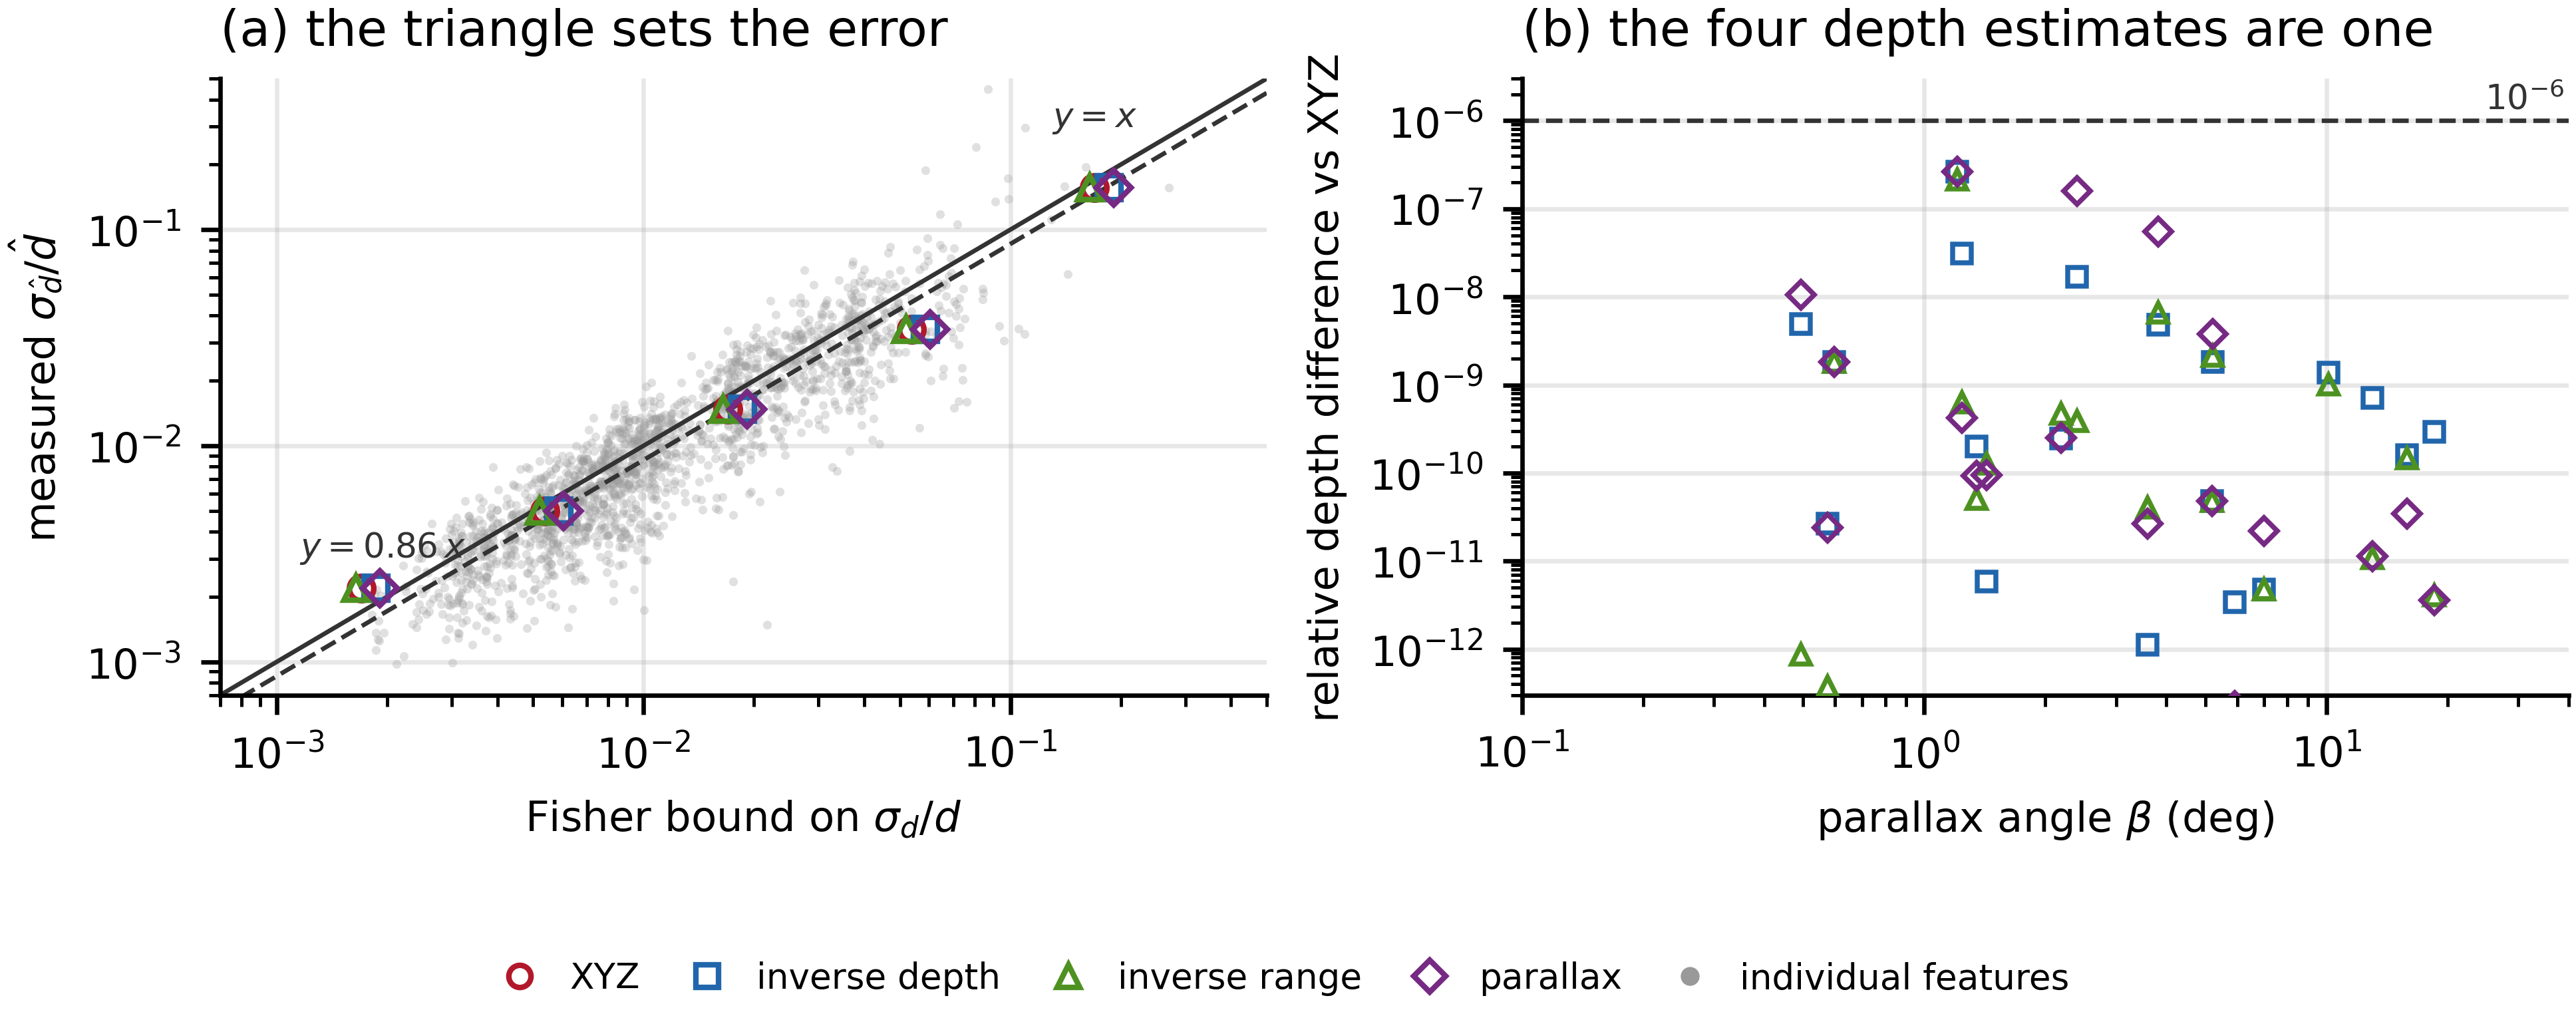
\includegraphics[width=\linewidth]{figures/real_depth.png}
\caption{(a) Measured depth sensitivity against the Fisher bound computed from each feature's own eight rays, over $1793$ features in nineteen windows of the TUM \texttt{fr1/xyz} sequence. Grey points are individual features; open markers are the medians of the bins of Table~\ref{tab:real-depth}, nudged horizontally by $4\%$ so that all four stay visible. The four charts lie on one band of slope one and normalisation $0.86$, the interquartile range of the ratio being $0.65$ to $1.10$. (b) The paired difference $|d_c-d_{\mathrm{XYZ}}|/d_{\mathrm{XYZ}}$ between each chart and XYZ, window by window; XYZ against itself is identically zero and so falls off the logarithmic axis. Every window, at every angle, lies below $3\times10^{-7}$, and the dashed line marks $10^{-6}$. What varies across the same windows is not the chart but the geometry: the Fisher bound of the retained features spans a factor of $150$.}
\label{fig:real-depth}
\end{figure}

If the chart does not set the depth error, the geometry of the triangle does. For one feature the eight bearing measurements give a $3\times3$ Fisher information matrix on its position, and the depth direction of its inverse gives the smallest standard deviation any unbiased estimator can reach. That bound contains no chart. Write $\sigma_d/d$ for it, computed at the measured point with the same $0.5$\,px.

Figure~\ref{fig:real-depth}(a) plots the measured spread against this bound. It runs from $0.002$ to $0.18$ and the measurement follows it across the whole range, with a median ratio of $0.86$ and an interquartile range of $0.65$ to $1.10$---consistent with one, given that a standard deviation from six draws has a relative standard error of $30\%$. The four charts give the same ratio to nine digits, because they give the same depth.

The bound is not the parallax angle. On the windows with a $1.3$\,cm baseline, a first-order propagation of one pixel through the triangle, $\sigma_{\mathrm{px}}/(f\tan\beta)$, predicts a relative error of $9.3\%$; the measurement gives $0.7\%$, a factor of fourteen. The reason is that a handheld camera also turns. A rotation displaces the image of a fixed point without moving the camera centre, and over eight frames that constrains depth as strongly as a baseline does; $\beta$ sees the translation and is blind to the rotation. The Fisher bound sees both and predicts $0.8\%$. A single scalar, whether it is a condition number or a parallax angle, does not summarise the conditioning of a three-dimensional point, and the failure is largest exactly where the parallax argument is usually made, at short baseline.

\subsection{The floor set by the sensor}

The last column of Table~\ref{tab:real-depth} is the error against the Kinect depth itself, and it does not follow the bound: it falls from $0.48$ to $0.013$ while the bound falls by a factor of a hundred, and at the small-bound end it saturates. The saturation is a property of the reference, not of the charts. A Kinect depth at $1.3$\,m carries a bias of about a centimetre, the motion-capture pose carries its own error, and both enter the anchor ray; the resulting floor is $1.3\%$ relative. Below $\beta\approx2^\circ$ the geometric term falls under it and the error against the sensor stops responding to the geometry. For the same reason the error against the sensor is three and a half times the bound at the median, while the spread of six draws is $0.86$ of it: the bias is real, common to all draws, and cancels in the spread but not in the error.

This is the honest boundary of the experiment. It measures the sensitivity of a point's depth to its observations on real geometry, real tracking and a real handheld motion, and it shows that the four charts share that sensitivity to nine digits. It cannot measure the absolute accuracy of a depth estimate on this sequence, because the reference is not accurate enough to say. A dataset with a laser-scanned reference would close that gap; the equality between charts does not depend on closing it.

\section{Discussion}
\subsection{Reconciling apparently conflicting reports}
The original ParallaxBA results, the short-baseline criticism of Zuo et al., and the large empirical gains reported since address different regimes and protocols. There is no logical contradiction:
\begin{itemize}[leftmargin=2em]
  \item A coordinate chart can yield well-scaled LM steps on many problems while remaining non-injective on a degenerate set.
  \item A positive-definite point-block information matrix and an identical reduced camera matrix are perfectly compatible, because the points are eliminated before the camera system is formed: Theorem~\ref{thm:main} makes this precise, and it is why single-block conditioning cannot serve as a BA diagnostic.
  \item A finite 100-iteration comparison can strongly favor Parallax without establishing a global convergence theorem.
  \item Extremely short-baseline three-dimensional configurations can expose angular sensitivity and numerical continuation issues even when a broad benchmark favors Parallax.
  \item Different initializations, stopping rules, damping metrics, and SfM acceptance decisions can dominate a small real experiment.
\end{itemize}
The correct response to the 2023 criticism is therefore not to dismiss it because some benchmark favors Parallax. Nor is it justified to infer from two short-baseline SfM experiments that Parallax is generally unsuitable for three-dimensional BA. The chart and the algorithm must be evaluated separately, and Theorem~\ref{thm:main} supplies the separation: it states which quantities cannot differ, which ones can, and why.

\subsection{What remains valuable about ParallaxBA}
Our analysis does not make ParallaxBA redundant, and Theorem~\ref{thm:main} says exactly where its value lies. Two of its statements are positive and non-trivial. First, the chart information matrix stays bounded while the XYZ one grows as $\omega^{-2}$; this is a preconditioning statement, not an information statement, because the two matrices are related by $I_q=D_q^{\T}I_XD_q$ and $\det I_q=(\det D_q)^{2}\det I_X$. Second, the chart trust region is stretched along depth by $d/B$ at $\beta=\pi/2$, so a fixed damping parameter does not freeze the depth direction at long range. The angle is also close to the measured quantity, which is a legitimate advantage for initialization and for robust loss geometry even though it does not change the Fisher information at a regular point.

What these properties do not provide is new image information, an invariant physical condition number, or an unconditional guarantee of metric-depth observability. The first two are excluded by Theorem~\ref{thm:main}(i)--(iii), which makes the rank and the reduced camera matrix chart invariants; the third is excluded by Proposition~\ref{prop:noninjective}. A claim that Parallax coordinates avoid singularity is therefore not a theorem about BA, whatever its two-dimensional auxiliary matrix says.

A practical implementation should report:
\begin{enumerate}[leftmargin=2em]
  \item the exact regularized residual and all domain guards;
  \item anchor-selection rules and distributions of $\omega$, $\sin\omega$, and scaled-ray norms;
  \item matched physical initial states and identical solver settings;
  \item both convergence flags and final objective quality;
  \item iteration/time comparisons conditioned on comparable solution quality;
  \item failure cases, rather than only aggregate medians.
\end{enumerate}

\subsection{Limitations}
This study has several boundaries. Theorem~\ref{thm:main} describes one linearization in one chart: it says nothing about the nonlinear convergence rate, the basin of attraction of a particular minimum, or the global topology of an atlas assembled from several charts. It also assumes a common residual, which holds for implementations that project the scaled ray but fails when a different residual or weighting is used; in that case rank and inertia survive, while the elementwise identity of $\mathcal S$ does not. Exact collinearity is a measure-zero event under continuous noise, although its neighborhood remains numerically relevant. The synthetic study uses one rig, one noise level, and one solver, so it establishes a mechanism rather than a population-level performance distribution; a corpus would be needed for the latter, and a corpus whose success criterion is depth-blind cannot supply it. The zero-ray result applies to the original ParallaxBA equation, not automatically to PMBA or other manifold extensions. The exact-alignment experiment is a rank statement about one configuration, not a statistical claim. Finally, the damped-trajectory results are specific to the damping rule tested; they do not exclude a switching rule that adapts to the actual trajectory.

\section{Conclusion}
Point coordinates are a congruence of the bundle-adjustment normal equations, so the reduced camera system a solver factorizes is identical elementwise in every regular chart. The camera block is not: an anchor-dependent chart enters the residual through the anchor poses as well as through the point, so $A_q=A+J_XG$ and $A_q^{\T}A_q$ differs from $A^{\T}A$ in both structure and values. The extra terms are $J_XG$, and $(I-P)$ is what removes them --- which is why the solve is unchanged while the matrix assembled on the way to it is not. What the chart remains free to choose is the damping metric and the domain, and neither carries information. A positive-definite auxiliary bearing/parallax matrix therefore coexists with non-identifiable Euclidean depth, and a condition number computed in chart coordinates measures those coordinates rather than the problem it is invoked to describe.

This is a refutation of an argument, not of a method. The two mechanisms the original analysis identifies are real, and we name them properly: the chart Hessian stays bounded while the XYZ one grows as $\omega^{-2}$, which is preconditioning, and at $\beta=\pi/2$ the trust region is stretched along depth by $d/B$, which is a damping geometry. Both survive, and both are worth having. What does not survive is the step from them to singularity avoided or to information gained --- nor the ordering that step would require, since inverse depth is the best-conditioned of the four charts at every angle in one scene examined here and the second worst in another.

The claims were checked where depth error is measurable rather than inferred from a residual. Four charts spanning seven orders of magnitude in $\kappa(H)$ produce the same physical Gauss--Newton iterates to $4\times10^{-14}$ and the same depth Cram\'er--Rao bound to $3\times10^{-10}$; at exact alignment they lose the same physical rank while the reduced camera system keeps full rank; a shared damping parameter moves the physical step by up to a factor of $4.9$, and the pulled-back metric restores agreement to $10^{-11}$; on a real handheld sequence the reduced system agrees to $9\times10^{-14}$ and the depth a chart returns for a feature to $3\times10^{-7}$, and that depth error follows a Fisher bound containing no chart to a ratio of $0.86$, while the parallax angle alone mispredicts it by a factor of fourteen. Singularity is a property of the problem rather than of the point parameterization. A chart can choose where it fails; Parallax coordinates choose well, and their claims are best evaluated at that level.

\section*{Reproducibility}
\label{sec:artifact}

\textbf{Code.} The artifact is at \url{https://github.com/Polar-vision/parallaxba-scaling}, under the MIT licence, with tag \texttt{v1.0} marking the state reported here. It carries the proof checks, the synthetic driver, the reproduction of Simulation~2, the two real-sequence tests, the scripts that draw every figure, and the six result files those scripts write.

\textbf{Supplementary material.} Three tables that support the identities of Sections~\ref{sec:damping}--\ref{sec:ba-theorem} without carrying the argument are collected in the supplementary document: rank bookkeeping for the collinear configuration (Table~S1), the damped steps along depth under a shared schedule (Table~S2), and the residuals of the exact identities (Table~S3).

\textbf{Data.} The synthetic problems are generated in process from the seeds fixed in the scripts, so no external corpus is read for them. The only third-party data are the TUM RGB-D sequence \texttt{fr1/xyz} \cite{sturm2012benchmark}: unpack it as \path{data/rgbd_dataset_freiburg1_xyz}, or point \texttt{--seq} in \path{real_depth_collapse.py} and the environment variable \texttt{TUM\_SEQ} in \path{real_invariance.py} somewhere else.

\textbf{Environment.} Python 3.11 with NumPy 1.26, OpenCV 4.11 and Matplotlib 3.10, single-threaded and without a GPU; \path{real_depth_collapse.py} runs in about six minutes. Every random draw is seeded, so a rerun reproduces the reported digits instead of approximating them.

\textbf{What writes what.} The six result files, all under \path{results/}, are \path{controlled_results.json} from the chart and continuation checks of Sections~\ref{sec:parallaxba}--\ref{sec:normalized-chart}, \path{ijrr_3d_ba_theorem.json} from the theorem checks of Section~\ref{sec:ba-theorem}, \path{synthetic_chart_experiment.json} from the synthetic study of Section~\ref{sec:synthetic}, \path{repro_sim2_ablation.json} from the reproduction of Section~\ref{sec:repro}, \path{real_invariance.json} from the invariance test of Section~\ref{sec:real}, and \path{real_depth_collapse.json} from the depth test of Section~\ref{sec:depth}. The six drivers, all under \path{code/}, pair one to one with those files: \path{verify_claims.py} for the chart and continuation checks, \path{verify_3d_ba_theorem.py} for the theorem, \path{synthetic_chart_experiment.py} for the synthetic study, \path{repro_sim2_ablation.py} for the re-run, and \path{real_invariance.py} with \path{real_depth_collapse.py} for the two real-sequence tests. The figures are drawn by \path{make_ba_theorem_figure.py}, \path{make_synthetic_figure.py} and \path{make_depth_figure.py}. \path{check_manuscript.py} reads the six result files, checks the numbers quoted above against them, and fails if one disagrees. No ground-truth accuracy, global-optimality, or controlled timing claim is inferred from data that do not measure it.

\section*{Declaration of conflicting interests}
The author declared no potential conflicts of interest with respect to the research, authorship, and/or publication of this article.

\section*{Funding}
This work was supported by the National Natural Science Foundation of China (grant no. T2600787) and the Natural Science Foundation of Shanxi Province (grant no. 202403021212106).

\section*{Author contributions}
ZZ conceived the study, developed the theory, implemented the code and the experiments, analysed the results, and wrote the manuscript. The author confirms sole responsibility for the content of this article.

\section*{Data availability}
The code, the six result files, and the scripts that redraw every figure are available at \url{https://github.com/Polar-vision/parallaxba-scaling}, tagged \texttt{v1.0} under the MIT licence. The TUM RGB-D sequence \texttt{fr1/xyz} used in Sections~\ref{sec:real}--\ref{sec:depth} is publicly available \cite{sturm2012benchmark}.

\bibliographystyle{apalike}
\bibliography{references}
\end{document}
